%base packages 
\documentclass[11pt]{article}
\usepackage[margin=1in]{geometry}
\usepackage{caption,multirow,etoolbox,color,enumerate,amsmath,dsfont,lscape,tocloft,booktabs,draftwatermark,array,tabularx,graphicx,pdflscape,subcaption}
\usepackage{setspace}
\setlength{\parskip}{0em}
\usepackage[bottom, flushmargin]{footmisc}
\usepackage[T1]{fontenc}
\usepackage[utf8]{inputenc}
\usepackage{lmodern}
\usepackage[english]{babel}
\usepackage[autostyle]{csquotes}
\makeatletter
\makeatother
\usepackage{float}
\SetWatermarkText{}\SetWatermarkLightness{0.85} \SetWatermarkScale{4}
\usepackage{appendix}
\usepackage{authblk}
\usepackage[format=hang,justification=raggedright,singlelinecheck=0,labelsep=period]{caption}
%[format=hang,justification=raggedright,singlelinecheck=0,labelsep=period]
%\usepackage[numbers,sort&compress]{natbib} %Use this set-up for numbered reference lists
\usepackage[authoryear]{natbib} %Use this set-up if you want an un-numbered reference list
%\usepackage{hypernat}

\usepackage[hyperfootnotes=false]{hyperref}
%\usepackage[dvipdfmx,hyperfootnotes=false]{hyperref}
%\usepackage[dvips,hyperfootnotes=false]{hyperref}
\hypersetup{colorlinks=true,linkcolor=blue,anchorcolor=blue,citecolor=blue,filecolor=blue,urlcolor=blue,bookmarksnumbered=true,pdfview=FitB} %
% % %DO NOT PLACE ANY PACKAGES AFTER THE HYPERREF SET UP
\usepackage{titling}

%-----------------------------------------------------------------------%
\begin{document}
\bibliographystyle{mla-good}


\title{Investigating the Inclusive-Performance Tradeoff in Agricultural Cooperatives: Evidence from Nepal\thanks{Copyright 2020 by Scott M. Miller (\href{scottmmiller@ufl.edu}{scottmmiller@ufl.edu}). All rights reserved. Readers may make verbatim copies of this document for non-commercial purposes by any means, provided this copyright notice appears on all such copies.} \thanks{This paper is made possible by the generous support of the American people through the United States Agency for International Development (USAID) and its Feed the Future Innovation Lab for Livestock Systems managed by the University of Florida and the International Livestock Research Institute. The contents are the responsibility of the author and do not necessarily reflect the views of USAID or the United States Government.}}


\author{Scott M. Miller \\ Food and Resource Economics Department \\ University of Florida}
\date{}

\sloppy
\maketitle

\vspace{2cm}
\begin{center}
\textit{Selected Paper prepared for presentation at the 2020 Agricultural \& Applied Economics Association \\ Annual Meeting in Kansas City, Missouri \\ July 26-28, 2020}  
\end{center}


\vspace{.5cm}

%------------------------------------------%
%\begin{abstract}
%Is there a tradeoff between inclusive membership and market performance in agricultural cooperatives? The answer to this question is critical for understanding the role that cooperatives play in agricultural development and poverty alleviation. However, studies on this topic have largely focused on membership criteria as the source of inclusion, overlooking the extent to which existing members are included in cooperative activities. This distinction is central to the challenge faced by cooperatives in which including a diverse membership may damage cooperative performance by increasing transaction costs but may also improve performance by pooling a quantity of inputs. In this essay, I use the Oaxaca-Blinder decomposition to further examine this relationship by analyzing i) whether there is a tradeoff between inclusive membership and market performance and ii) whether this tradeoff is explained by differences in observable characteristics or differences in the ability to translate those characteristics into results.
%\end{abstract}
%------------------------------------------%

\pagenumbering{gobble}
\clearpage
\renewcommand{\cftsecleader}{\cftdotfill{\cftdotsep}}

%\tableofcontents
%\clearpage

\doublespacing
\thispagestyle{plain}
\pagenumbering{arabic}
\setcounter{page}{1}

%-----------------------------------------------------------------------%
\section{Introduction} \label{sec:intro}
% Hook
Two-thirds of the world's poorest households live in rural areas and depend on agriculture for their livelihoods \citep{k_fuglie_harvesting_2019}. Tackling poverty, hunger and malnutrition require drastically increasing the production and commercialization of smallholder agricultural producers \citep{fischer_smallholder_2014,world_bank_world_2008}. Despite the important role that agriculture plays in reducing poverty \citep{k_fuglie_harvesting_2019}, rural markets in developing countries are often rife with constraints that limit the ability of smallholders to gain from formal markets \citep{ashby_investing_nodate,p_kristjanson_notitle_2014}. These constraints include poor infrastructure, weak communication channels and long distances between market actors that lead to high transaction costs, weak bargaining power and information asymmetry \citep{aker_information_2010,barrett_smallholder_2008,key_transactions_2000,staal_smallholder_1997}. 

In the face of severe market constraints, agricultural cooperatives often arise in an effort to increase bargaining power, decrease transaction costs, and help achieve scale economies in marketing \citep{markelova_collective_2010,rondot_agricultural_2001,staal_smallholder_1997,csaki_reaching_2003}. By exploiting the potential of collective action, cooperatives provide the opportunity for smallholders to access markets that may otherwise be inaccessible, pool resources to overcome financial constraints, increase communication flows and collectively negotiate with buyers to receive better prices \citep{poole_review_2010}. However, cooperatives do not eliminate the source of market constraints. Rather, collective action shifts these burdens from individual market actors to the cooperatives themselves. The effectiveness of cooperatives in raising smallholder market engagement depends on how well cooperatives manage the challenge of internally coordinating sales among a large group of individual market actors \citep{mullally_impact_2020}. Evidence suggests that some farmer organizations are able to successfully overcome this challenge, generating large and inclusive benefits for their members \citep{narrod_publicprivate_2009,tadesse_mobile_2015,wollni_farmers_2007}. Others largely fail in this effort, resulting in weak market performance, heterogeneous benefits or dissolving participation among their members \citep{aflagah_cheap_2019,bernard_reaching_2009, casaburi_loyalty_2015}. 

% Question 
One aspect that may contribute to this disparity is the relationship between inclusive membership and market performance in agricultural cooperatives. This relationship has been highlighted as an unresolved conflict in the cooperative literature, where organizations struggle to balance social inclusion with the challenge of coordinating activities among a diverse membership \citep{bernard_reaching_2009,world_bank_world_2008}. Determining the extent of this inclusive-performance tradeoff is essential to understanding the role that cooperatives play in agricultural development and poverty alleviation. Studies on this topic have largely focused on cooperative membership as the source of inclusion, overlooking the extent to which existing members are included in group activities. This distinction is central to the challenge faced by cooperatives. Including a diverse membership may damage cooperative performance by increasing transaction costs \citep{world_bank_world_2008}, but including a large number of existing members in a given activity may improve performance by pooling a larger quantity of inputs \citep{aflagah_cheap_2019}. 

% Antecedents
Prior studies argue that cooperatives with performance oriented membership rules are better able to reduce the transaction costs associated with coordination and the management of group activities \citep{bernard_reaching_2009}. This issue has received considerable attention as these rules tend to exclude the most vulnerable households from receiving the benefits associated with cooperative membership \citep{world_bank_world_2008}. Conversely, organizing bulk sales of members' output can be viewed as a critical mass coordination game, where a larger number of participants can improve the bargaining position of the cooperative by increasing the quantity of marketable output \citep{aflagah_cheap_2019}. If cooperatives are able to successfully manage the coordination challenge associated with increased group size, organizations that include a larger share of their membership in activities may be able to generate broader benefits. %CM: You've laid out why membership size may have an ambiguous relationship with cooperative performance. But what about your particular question, i.e. inclusiveness conditional on being a member? If you see the same arguments applying to the extensive (membership size) and intensive (inclusiveness conditional on membership) with regards to cooperative performance, that's fine. But you should make that point. I think it kind of comes down to what the shape of the MC and MB curves are. Does the latter go up with inclusiveness because of bargaining power? Is the former flat, U-shaped, half-U?

% Value Added
In this paper, I examine the inclusive-performance tradeoff across two dimensions: extensive and intensive inclusion. The former describes the inclusion of a diverse set of households in a cooperative's membership, while the latter describes the extent to which existing members are included cooperative activities. First, I analyze the relationship between inclusive membership and market performance across the extensive and intensive dimensions. I then use the \citet{oaxaca_male-female_1973}-\citet{blinder_wage_1973} decomposition to determine whether these relationships are best explained by differences in observable characteristics or differences in the returns to those characteristics. My population of interest are smallholder goat producers in rural Nepal, all of whom are women and members of agricultural cooperatives. The data used in this study covers 2,856 households across 108 smallholder livestock cooperatives in Nepal. 

I find that cooperatives that include a larger share of illiterate and low asset holding farmers in their membership perform significantly worse than their less inclusive counterparts. While this result is consistent with the inclusive-performance tradeoff, I also find that cooperatives that include a larger share of their members in group activities perform better than their less inclusive counterparts. Both results are largely driven by differences in returns to the observable characteristics between the most and least inclusive cooperatives. This suggests that both extensive and intensive inclusion have a meaningful, but opposite, impact on a cooperative's ability to achieve market performance. Finally, my results indicate that these results are largely not explained by differences in observable characteristics between the two groups. %CM: Ok, so you do both dimensions of inclusiveness. That's great. I think my point above still stands though.  


%-----------------------------------------------------------------------%
\section{Background} \label{sec:background}

In Nepal, where 68 percent of the population depends on agriculture for their livelihood %CM: Maybe establish the context in the intro. Otherwise the intro of Heifer in the Background section is a little bit awkward
\citep{international_labor_organization_ilo_2016}, goats are a common source of income and nutrition. This is particularly true in rural areas, where almost every household owns a least a few goats \citep{upreti_food_2009}. In recent years, urbanization and rising incomes have lead to a higher demand for goat meat, but a poorly functioning value chain has left smallholder producers, most of whom are women, unable to benefit \citep{ashby_investing_nodate,choudhary_pro-poor_2011,gurung_empowering_2015}. Smallholders face high transaction costs, weak bargaining power and a lack of communication infrastructure that limit their ability to access and gain from formal output markets \citep{ashby_investing_nodate,p_kristjanson_notitle_2014}. As a result, domestic production has been unable to keep up with rising demand, leading to higher imports from India and Tibet \citep{heifer_international_nepal_study_2012}.

Many agricultural policy and rural development plans in Nepal have promoted agricultural cooperatives as a means of supporting smallholder producers \citep{agricultural_development_strategy_agricultural_2015}. Non-governmental organizations, including Heifer Project International in Nepal (HPIN), have made recent efforts to strengthen the goat value chain by organizing producer cooperatives. HPIN’s programs give women livestock and extensive training. Beneficiaries are then organized into self-help groups of around 20-30 female members. Once self-help groups in a given area are sufficiently organized, they are combined into larger producer cooperatives \citep{janzen_short-term_2018}.

% This follows closely from the VCC Pre-Analysis Plan. In the full dissertation,
In Nepal, the majority of goats are consumed locally after sale to a local collector who pools animals from small producers, or to a local butcher \citep{heifer_international_nepal_study_2012}. For goats that are marketed outside their original communities, the commercial value chain links producers, local collectors, regional traders who pool animals purchased from collectors, processors and retailers, and finally consumers who are primarily located in urban markets like the Kathmandu Valley \citep{heifer_international_nepal_study_2012}. A collector looking to buy goats from smallholder producers who are not affiliated with a cooperative would likely have to conduct individual negotiations, sometimes making multiple visits per home \citep{heifer_international_nepal_study_2012, staal_smallholder_1997}. After agreeing to terms with producers, the collector would still have to coordinate transportation. Bargaining with many small producers and managing logistics may inflate transaction costs and dissuade collectors from dealing with smallholders. In contrast, a collector purchasing through a cooperative need only negotiate with a single entity and can leave sales coordination to cooperative managers. 

The cooperatives included in my data appear to struggle with coordinating goat sales in a way that is broadly inclusive of members. Although officers from 86\% cooperatives in my data stated that their organizations coordinated goat sales, only 35\% of households received information about a cooperative sale in the six-months prior to data collection. My baseline data suggest that these cooperatives largely communicate in person. Among the households that did receive price and sales information, half indicate that they did so by word of mouth, nearly 75\% indicated receiving this information through SHG meetings, while only 19\% did so by phone call and less than 1\% via short message service (SMS).

The failure to transmit information about sales could be the result of meeting infrequently, as nearly all households state that SHG meetings happen monthly or less while nearly two-thirds indicate that cooperative meetings take place every two months or less. Distance to meetings points could be a barrier to more frequent interactions, as cooperative members state that it takes approximately 90 minutes to travel to and from cooperative meetings, on average. Road quality, access to transportation, and distance between cooperative members were identified by 90\%, 93\%, and 83\% of cooperative leaders, respectively, as limiting communication.

The difficulties associated with word-of-mouth communication emphasize the transaction costs associated with including new members in the cooperative as well as existing members in group activities. Given that cooperatives average about 500 members each, calling all members or confirming that all receive a text message may seem more onerous than holding a meeting. This issue may directly affect market performance if cooperatives are failing to consider the entire inventory at their disposal by not including a large share of members in group sales. 

%-----------------------------------------------------------------------%
\section{Data} \label{sec:data}
In this paper I use a cross-sectional dataset covering 2,856 goat producing households across 108 female smallholder livestock cooperatives in Nepal. The cooperatives in this sample are spread across four of five development regions in Nepal, specifically the East, Central, West and Mid-Western Development regions. All cooperatives operate in either the low-land Terai or mid-Hills. Figure (\ref{map}) shows the study area covered in the sample, which includes cooperatives from 24 districts across Nepal. The cooperatives included in the study were selected by HPIN and include all existing livestock marketing cooperatives the organization helped form prior to 2017.

\begin{figure}[!h]
    \caption{Study Area}
    \label{map}
    \noindent \centering 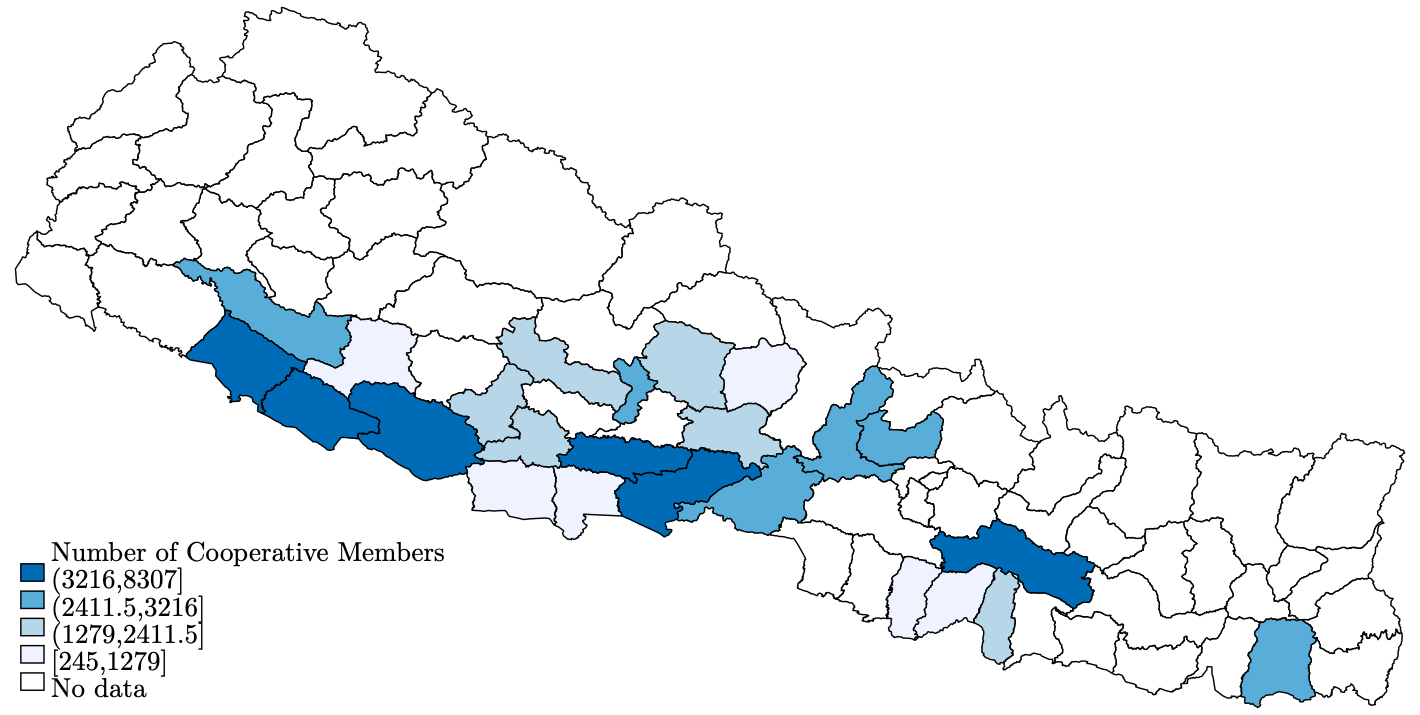
\includegraphics[width=.9\textwidth,trim=4 4 4 4,clip]{StudyMap.png}
\end{figure}

This dataset consists of two separate surveys - one with cooperative leaders and another with general members.  %CM: If this feature of our data is unique in the co-op literature, you could emphasize it a bit more in the intro.
I refer to these surveys as the cooperative leader and household survey, respectively. The cooperative leader survey is comprised of interviews from three officers in each cooperative. To obtain a representative sample for the household survey, HPIN and cooperative leaders generated complete cooperative rosters. From these comprehensive lists, a random sample of 2,856 households across 108 %CM: or 109?
cooperatives was drawn to participate in the household survey. The data were collected from the sample in January 2018 using Android tablets and Open Data Kit.

\singlespacing
% Summary Stats Table
\newcolumntype{Y}{>{\centering\arraybackslash}X}
\begin{table}[!h]
  \centering
  \caption{Summary Statistics}
  \label{table:E1_summary}
  \scalebox{.8}{
  \begin{tabularx}{1.2\linewidth}{l*{7}{Y}}
\hline Cooperative-Level Variables & N & Mean & sd & Min & Max\\
\noalign{\smallskip}\hline \noalign{\smallskip}
Number of members (count) & 107.00 & 568.64 & 375.77 & 11.00 & 2,600.00\\
Total revenue over last 6-months (USD) & 106.00 & 3,934.92 & 7,555.17 & 0.00 & 65,709.51\\
Cooperative has an initial membership fee (0/1) & 107.00 & 0.93 & 0.26 & 0.00 & 1.00\\
Size of initial membership fee (USD) & 108.00 & 2.22 & 3.86 & 0.00 & 35.64\\
Share of members the attending last general assembly (count) & 108.00 & 0.64 & 0.27 & 0.00 & 1.00\\
Size of management committee (count) & 107.00 & 10.46 & 1.78 & 7.00 & 15.00\\
Number of services offered (count) & 107.00 & 8.04 & 2.57 & 2.00 & 17.00\\
Coordinates goat sales (0/1) & 108.00 & 0.59 & 0.39 & 0.00 & 1.00\\
Offers loans to members  (0/1) & 108.00 & 0.97 & 0.07 & 0.55 & 1.00\\

  \end{tabularx}}
  \scalebox{.8}{
  \begin{tabularx}{1.2\linewidth}{l*{7}{Y}}
\hline Household-Level Variables & N & Mean & sd & Min & Max\\
\noalign{\smallskip}\hline \noalign{\smallskip}
Age (years) & 2,856.00 & 40.40 & 11.56 & 20.00 & 83.00\\
Literacy (0/1) & 2,853.00 & 0.72 & 0.45 & 0.00 & 1.00\\
Length of membership (years) & 2,856.00 & 3.04 & 1.84 & 0.00 & 9.00\\
Round-trip travel time to cooperative meetings (minutes) & 2,856.00 & 91.58 & 103.41 & 0.00 & 420.00\\
Voted in elections in last 2-years (0/1) & 2,856.00 & 0.09 & 0.29 & 0.00 & 1.00\\
Contacted about cooperative sales in last 6-months (0/1) & 2,856.00 & 0.35 & 0.48 & 0.00 & 1.00\\
Contacted about cooperative activities in last 6-months (0/1) & 2,856.00 & 0.38 & 0.49 & 0.00 & 1.00\\
Primary activity is agriculture (0/1) & 2,856.00 & 0.71 & 0.45 & 0.00 & 1.00\\
Total number of goats owned (count) & 2,856.00 & 5.76 & 4.95 & 0.00 & 69.00\\
Sold goats in the last 12-months (0/1) & 2,856.00 & 0.48 & 0.50 & 0.00 & 1.00\\
Annual number of goats sold (count) & 2,856.00 & 1.12 & 1.73 & 0.00 & 10.00\\
Annual revenue per goat (USD) & 2,856.00 & 41.91 & 53.56 & 0.00 & 742.50\\
\hline
\multicolumn{6}{@{}p{1\textwidth}}
{\textit{Notes}: }
  \end{tabularx}}
\end{table}
\doublespacing

Table (\ref{table:E1_summary}) provides summary statistics from my data. The average cooperative in my sample has 569 members, and a revenue of over \$3,800 USD. While 93\% of cooperatives have an initial membership fee, the average cooperative charges \$2.22 USD. At the last general assembly meeting prior to data collection, only 64\% of members were in attendance, on average. At the household level, the average cooperative member is 42 years old, roughly 80\% of whom are literate. The average member has been a member of their cooperative for 3 years. On average, members have attended more than five self-help group meetings in the 6-months prior to data collection and attended fewer than two cooperative meetings over this period. Members indicate an average round-trip travel time to the cooperative of more than 90 minutes. While nearly 70\% of members indicate that they participate in the cooperative's general meeting, fewer than 10\% have voted in cooperative elections in the last 2-4 years. Roughly 35\% of members were contacted about cooperative organized livestock sales in the 6-months prior to data collection and 38\% were contacted about non-sale related cooperative activities. 
%CM: depending on how it features in your later analysis, you might put something about savings or credit in the individual summary stats.

\singlespacing
% Summary Stats Table
\newcolumntype{Y}{>{\centering\arraybackslash}X}
\begin{table}[H]
  \centering
  \caption{Cooperative Services}
  \label{table:E1_services}
  \scalebox{.7}{
  \begin{tabularx}{1.3\linewidth}{lccc}
\hline \noalign{\smallskip} & Share of cooperatives & Share of members & Share of members\\
 & offering service & aware of service & using service\\
 &  &  & (where offered)\\
\noalign{\smallskip}\hline \noalign{\smallskip}Accept savings deposits (0/1) & 0.97 & 0.98 & 0.96\\
Offer loans (0/1) & 0.91 & 0.97 & 0.33\\
Provide goat price information (0/1) & 0.87 & 0.58 & . \\
Coordinate sales of goats to traders (0/1) & 0.86 & 0.60 & 0.14\\
Provide assistance with animal husbandry (0/1) & 0.79 & 0.55 & 0.64\\
Give dividend payments to owners of cooperative shares (0/1) & 0.66 & 0.45 & 0.13\\
Provide access to veterinary services (0/1) & 0.65 & 0.42 & 0.87\\
Provide assistance with business planning (0/1) & 0.62 & 0.38 & 0.28\\
Sell or help members access livestock insurance (0/1) & 0.41 & 0.47 & 0.43\\
Help members access bank loans & 0.37 & 0.32 & 0.62\\
Sell fertilizer (0/1) & 0.21 & 0.20 & . \\
Sell seed (0/1) & 0.16 & 0.19 & 0.55\\
Sell consumer goods, such as food (0/1) & 0.13 & 0.13 & 0.50\\
Sell animal feed (0/1) & 0.11 & 0.14 & 0.40\\
Sell or rent agricultural or livestock tools (0/1) & 0.04 & 0.05 & 0.27\\
Sell pesticide (0/1) & 0.03 & 0.07 & 0.46\\
\noalign{\smallskip}\hline
\multicolumn{4}{@{}p{1.3\textwidth}}
{\textit{Notes}: This table displays the share of cooperatives offering a given service, the share of members who are aware that their cooperative offers this service and the share of members who have used each service in the year prior to data collection (among the members whose cooperative offers them). There is no data available on the share of members who were assisted by their cooperative in accessing a bank loan or the share of members who received goat price information.}
  \end{tabularx}}
\end{table}
\doublespacing

Table (\ref{table:E1_services}) displays the various services that cooperatives offer in this context. The first column indicates the share of cooperatives that offer each service, the second column displays the share of members that believe their cooperative offers that service and the last column indicates the share of members using a given service in the cooperatives that offer it. The most common services offered by the cooperatives in my sample are accepting savings deposits (97\%), offering loans to members (91\%), providing goat price information (87\%) and coordinating goat sales with traders (86\%). Among the sample of cooperative members, there is a large disparity in awareness and participation between the various services. While almost all members are aware of and save money through the cooperative, only 14\% of members sold at least one goat through the cooperative in the year prior to data collection and a third of members had an outstanding loan from the cooperative at the time of data collection.


%-----------------------------------------------------------------------%
\section{Empirical Strategy} \label{sec:E1_emp}

%-----------------------------------------------------------------------%
\subsection{Theoretical Framework} \label{sec:E1_theory}

The \citet{oaxaca_male-female_1973}-\citet{blinder_wage_1973} decomposition allows me to separate the observed average outcomes between the most and least inclusive cooperatives into an explained and an unexplained component. Although decomposition methods typically do not provide causal estimates, this approach closely follows the program evaluation literature, where the `unexplained' portion of the gap (i.e. returns to characteristics) is analogous to a treatment effect \citep{n_fortin_notitle_2011}.

For example, suppose that the relationship between the outcome for farmer $i$, $Y_i$, and a vector of the determinants of performance, $\mathbf{X}_i$, can be written as

\begin{equation} \label{eq:E1_1}
    Y_i = \beta \mathbf{X}_i + \varepsilon_i
\end{equation}  

%CM: Be clear what \beta is. 
Given that the most and least inclusive cooperatives likely differ in their ability to translate members' characteristics into performance, I will allow for different values of $\beta$ for each group. Using the group-specific parameters, the difference between average outcomes for the most and least inclusive cooperatives is written as:

\begin{equation} \label{eq:E1_2}
        \overline{Y}_{m} - \overline{Y}_{\ell} =  \beta_{m}\overline{\mathbf{X}}_{m} - \beta_{\ell}\overline{\mathbf{X}}_{\ell}
\end{equation}  

where $m$ and $\ell$ represent the most and least inclusive cooperatives, respectively. Rearranging this equation by adding and subtracting $\beta_{\ell}\overline{\mathbf{X}}_{m}$ on both sides gives:
\begin{subequations}
    \begin{align}
        \overline{Y}&_{m} - \overline{Y}_{\ell} \label{eq:E1_3a} \\
                &= \beta_{\ell}[\overline{\mathbf{X}}_{m} - \overline{\mathbf{X}}_{\ell}] \label{eq:E1_3b} \\
                &+ \overline{\mathbf{X}}_{m}[\beta_{m} - \beta_{\ell}] \label{eq:E1_3c}
    \end{align}
\end{subequations}  

Here, (\ref{eq:E1_3b}) is the explained component (weighted by the coefficients for producers in the least inclusive cooperatives), which is the difference between the average outcomes that producers in the least inclusive cooperatives actually receive, given their characteristics, and what they could receive if their characteristics matched those of producers in the most inclusive cooperatives. %CM: Importantly, this interpretation holds regardless of whether the conditional mean is linear in parameters, because the regression line always go through the sample average (Ybar and Xbar). In other words, not only do you not have to identify a causal effect, you also don't need a linear conditional mean for this decomposition to be useful.
Line (\ref{eq:E1_3c}) is the unexplained component (weighted by the characteristics of producers in the most inclusive cooperatives), which is the difference between what producers in the most inclusive cooperatives actually receive and what they would receive if they had equivalent returns to their characteristics as those in the least inclusive cooperatives.

%-----------------------------------------------------------------------%
\subsection{Estimating the Oaxaca Decomposition} \label{sec:E1_est}

An important aspect of this analysis is determining whether the performance gap between the most and least inclusive cooperatives is best explained by observable differences across groups or unobservable differences in the ability to translate characteristics into performance. The Oaxaca-Blinder decomposition provides a useful framework for understanding this relationship. However, characteristics at both the individual- and cooperative-level are likely to be important factors in explaining market performance. Therefore, I expand the above framework to include two separate vectors of attributes: one institutional and one individual, such that

\begin{equation} \label{eq:E1_4}
   Y_{ij} = \mathbf{X}_i^{\prime}\beta + \mathbf{Z}_j^{\prime}\gamma + \varepsilon_{ij}
\end{equation}  

where $Y_{ij}$ is the outcome of interest for individual $i$ who is a member of cooperative $j$, $\mathbf{X}_i$ is a vector of individual attributes and $\mathbf{Z}_j$ is a vector of institutional attributes. Additionally, I include a district dummy to account for location-specific effects and cluster $\varepsilon_{ij}$ at the cooperative level. Allowing for the most and least inclusive cooperatives to differ in their ability to translate individual and institutional attributes into market performance, equation (\ref{eq:E1_2}) becomes

\begin{equation} \label{eq:E1_5}
        \overline{Y}_{m} - \overline{Y}_{\ell} =  (\beta_{m}\overline{\mathbf{X}}_{m} - \beta_{\ell}\overline{\mathbf{X}}_{\ell}) + (\gamma_{m}\overline{\mathbf{Z}}_{m} - \gamma_{\ell}\overline{\mathbf{Z}}_{\ell})
\end{equation}  

Rearranging equation (\ref{eq:E1_5}) by adding and subtracting $(\beta_{m}\overline{\mathbf{X}}_{\ell} + \gamma_{m}\overline{\mathbf{Z}}_{\ell})$ on both sides gives my final decomposition equation:
\begin{subequations}
    \begin{align}
        \overline{Y}&_{m} - \overline{Y}_{\ell} \label{eq:E1_6a} \\
        &= (\beta_{\ell}[\overline{\mathbf{X}}_{m} - \overline{\mathbf{X}}_{\ell}] + \gamma_{\ell}[\overline{\mathbf{Z}}_{m} - \overline{\mathbf{Z}}_{\ell}]) \label{eq:E1_6b} \\
        &+ (\overline{\mathbf{X}}_{m}[\beta_{m} - \beta_{\ell}] + \overline{\mathbf{Z}}_{m}[\gamma_{m} - \gamma_{\ell}]) \label{eq:E1_6c}
    \end{align}
\end{subequations}  

As in the example in section \ref{sec:E1_theory}, equation (\ref{eq:E1_6b}) is the explained component (weighted by the coefficients for individual and institutional characteristics in the least inclusive cooperatives). The first part of this equation, $\beta_{\ell}[\overline{\mathbf{X}}_{m} - \overline{\mathbf{X}}_{\ell}]$, is the difference between average outcomes that producers in the least inclusive cooperatives actually receive, given their characteristics, and what they might receive if their characteristics were changed to match those of producers in the most inclusive cooperatives. The second part of this equation, $\gamma_{\ell}[\overline{\mathbf{Z}}_{m} - \overline{\mathbf{Z}}_{\ell}]$, is the cooperative-level analog to the first part. This represents the average outcomes that producers in the least inclusive cooperatives actually receive, given their cooperative's characteristics, and what they could receive if their cooperative's characteristics were changed to match those of the most inclusive cooperatives. This is the portion of the gap that is due to individual and institutional characteristics, respectively.

Equation (\ref{eq:E1_6c}) is the unexplained component (weighted by the individual and institutional characteristics of the most inclusive cooperatives). The first part of this equation, $\overline{\mathbf{X}}_{m}[\beta_{m} - \beta_{\ell}]$, is the difference in what producers in the most inclusive cooperatives actually receive and what they could receive if they had equivalent returns to their characteristics as those in the least inclusive cooperatives. The institutional analog, $\overline{\mathbf{Z}}_{m}[\gamma_{m} - \gamma_{\ell}]$, is the difference that producers in the most inclusive cooperatives actually receive and what they could receive if they had equivalent returns to institutional characteristics as those in the least inclusive cooperatives. This is the portion of the gap that is due to individual and institutional returns, respectively.

%-----------------------------------------------------------------------%
\section{Results}

\subsection{Determinants of Intensive Inclusion}

Table (\ref{table:E1_inclusion}) displays the relationship between members' characteristics and the extent to which they are included in cooperative activities. Columns 1-4 report the results of logit regressions on each of the following binary indicators of inclusion: whether the member currently holds a leadership role in the cooperative, whether the member received information about a cooperative organized goat sale in the last year, whether the member received information about a cooperative organized activity other than a sale in the last year, whether the member voted in cooperative elections in the last 2-4 years and whether the household currently has a loan outstanding from the cooperative. 

\singlespacing
% Summary Stats Table
\newcolumntype{Y}{>{\centering\arraybackslash}X}
\begin{table}[H]
  \centering
  \caption{Determinants of inclusion (logit: marginal effect at mean of independent variable)}
  \label{table:E1_inclusion}
  \scalebox{.65}{
  \begin{tabularx}{1.45\linewidth}{llllll} \hline
 & (1) & (2) & (3) & (4) & (5) \\
Variables & Leadership & Received sale & Received non-sale & Voted in & Received \\
 & role (0/1) & information (0/1) & information (0/1) & election (0/1) & loan (0/1) \\
\hline
 &  &  &  &  &  \\
Literacy (0/1) & 2.304*** & 0.479*** & 0.508*** & 0.174 & 0.204* \\
 & (0.397) & (0.104) & (0.099) & (0.170) & (0.110) \\
Age (years) & -0.002 & -0.013*** & -0.004 & -0.016** & -0.015*** \\
 & (0.008) & (0.004) & (0.004) & (0.007) & (0.004) \\
Number of household members (count) & -0.060* & 0.034** & -0.007 & -0.022 & -0.009 \\
 & (0.035) & (0.015) & (0.015) & (0.027) & (0.017) \\
Total number of goats owned (count) & 0.029** & 0.061*** & 0.021** & 0.016 & 0.006 \\
 & (0.013) & (0.009) & (0.008) & (0.013) & (0.010) \\
Length of membership (years) & -0.190*** & -0.133*** & 0.000 & 0.197*** & 0.095*** \\
 & (0.047) & (0.024) & (0.022) & (0.033) & (0.024) \\
Round-trip travel time to cooperative meetings (minutes) & 0.001** & -0.002*** & -0.002*** & -0.002** & -0.002*** \\
 & (0.001) & (0.000) & (0.000) & (0.001) & (0.000) \\
Number of cooperative members (count) & -0.001*** & 0.001*** & 0.000 & 0.000 & 0.000 \\
 & (0.000) & (0.000) & (0.000) & (0.000) & (0.000) \\
Constant & -3.429*** & -0.795*** & -0.601** & -2.237*** & -0.588** \\
 & (0.597) & (0.246) & (0.237) & (0.402) & (0.265) \\
 &  &  &  &  &  \\
 Observations & 2,829 & 2,829 & 2,829 & 2,829 & 2,829 \\ \hline
\multicolumn{6}{@{}p{1.45\linewidth}}
{\textit{Notes}: Results from a logit regression, reporting the marginal effects at the mean of each independent variable. Standard errors in parentheses (*** p$<$0.01, ** p$<$0.05, * p$<$0.1). }
  \end{tabularx}}
\end{table}
\doublespacing

These results indicate that cooperatives may be including members to different degrees based on their characteristics. Literate cooperative members are significantly more likely to hold a leadership role, to have received sale and non-sale information from the cooperative, and to have an outstanding loan from the cooperative. Interestingly, older members are significantly less likely to be included across four of the five outcomes, with the exception being the receipt of information about non-sale activities. Members who own a larger number of goats are significantly more likely to hold a leadership role and receive information regarding cooperative sales and activities. Although those that have been members of the cooperative longer are less likely to be in a leadership role or to receive sale information, these members are more likely to have voted in cooperative elections and more likely to have a loan from the cooperative. Additionally, members who live farther away from the cooperative are significantly less likely to be included across four of the five outcomes.  


\subsection{Group Definitions}

In this subsection I describe how I split cooperatives into the most and least inclusive groups and present the average performance gap along each outcome used in my analysis. First, I define inclusive membership based on criteria for allowing a diverse membership to participate in the cooperative (extensive inclusion): literacy, the share of members who own fewer than the sample median number of goats, the coefficient of variation on goats owned per member and the size of the cooperative membership fee. To sort cooperatives along the literacy dimension, I calculate the share of members in each cooperative that are nonliterate and split this variable at the median value. Cooperatives whose share of nonliterate members is above the sample median are placed into the `most inclusive' group and those at or below the median share are placed into the `least inclusive' group. For the share of members below the median number of goats owned, I calculate the median number of goats owned for the full sample and the share of each cooperative's members that own fewer than this number of goats. I then split this variable at the median value, sorting cooperatives that are above the median value into the most inclusive group and those at or below the median into the least inclusive group. Additionally, I calculate the coefficient of variation on the number of goats owned per member within each cooperative and split cooperatives at the median value of this statistic, with those above the median value placed into the most inclusive group. Finally, I split cooperatives based on the size of the membership fee required to join the cooperative, sorting those with a membership fee below the median value into the most inclusive group. 
%CM: If and when we do our follow-up, it seems like we should ask about criteria for becoming a member.

I then define of inclusive membership based on the extent to which existing members are included in various group activities (intensive inclusion). I split cooperatives at the median value of: the share of members receiving information about a cooperative organized goat sale, the share of members receiving information about a cooperative organized activity other than a sale, the share of members that currently have an outstanding loan from the cooperative and the share of members that voted in cooperative elections in the last 2-4 years. Across each dimension, I follow the same process described above, sorting cooperatives above the median value of each statistic into the `most inclusive' group, and those at or below the median value into the least inclusive group.

\subsection{Outcomes and Performance Gaps}
%CM: give the units for the index impacts (standard deviations, right?)

The outcomes of interest in this study are defined as follows: the revenue received by each member from selling goats through the cooperative, the number of goats sold by each member through the cooperative, the value of outstanding cooperative loans that each member holds and a cooperative benefits index.\footnote{For cooperative goat revenue and the number of cooperative goats sold, I include only members who sold at least one goat in the year prior to data collection. As listed in table (\ref{table:E1_summary}), 48\% of all members sold at least one goat during this period. Among this subsample, XX\% sold at least one goat through the cooperative. Members who sold goats but did not sell through the cooperative have a value of zero for both variables. Therefore, the outcomes for these variables should be viewed as the outcome among goat-selling members.} The cooperative benefits index is an inverse covariance weighted index of the three outcome variables described above, following the apporach outlined in \citet{anderson_multiple_2008}.

\singlespacing
% Summary Stats Table
\newcolumntype{Y}{>{\centering\arraybackslash}X}
\begin{table}[H]
  \centering
  \caption{Average performance gap between the most and least inclusive cooperatives}
  \label{table:E1_gap}
  \scalebox{.65}{
  \begin{tabularx}{1.5\linewidth}{lllll}
\hline \noalign{\smallskip}Group Definition (split at median) & Cooperative goat & Cooperative goats & Cooperative loan & Cooperative benefits\\
 & revenue (USD) & sold (count) & amount (USD) & index\\
 \noalign{\smallskip}\hline \\
  & (N= ) & (N= ) & (N= ) & (N= ) \\
\textbf{Extensive Inclusion} & & & & \\ 
\noalign{\smallskip}Percentage of non-literate members & -10.38 & -0.13** & -59.81 & -0.21***\\
 & \begin{footnotesize}(6.87)\end{footnotesize} & \begin{footnotesize}(0.06)\end{footnotesize} & \begin{footnotesize}(40.75)\end{footnotesize} & \begin{footnotesize}(0.07)\end{footnotesize}\\
\noalign{\smallskip}Percentage of members below the median number of goats owned & -47.99*** & -0.47*** & 20.68 & -0.24***\\
 & \begin{footnotesize}(6.72)\end{footnotesize} & \begin{footnotesize}(0.06)\end{footnotesize} & \begin{footnotesize}(40.70)\end{footnotesize} & \begin{footnotesize}(0.07)\end{footnotesize}\\
\noalign{\smallskip}Coefficient of variation on members' goats & -1.04 & -0.04 & 39.84 & -0.05\\
 & \begin{footnotesize}(6.78)\end{footnotesize} & \begin{footnotesize}(0.06)\end{footnotesize} & \begin{footnotesize}(40.69)\end{footnotesize} & \begin{footnotesize}(0.07)\end{footnotesize}\\
\noalign{\smallskip}Size of membership fee & 9.40 & 0.08 & -59.76 & -0.02\\
 & \begin{footnotesize}(6.79)\end{footnotesize} & \begin{footnotesize}(0.06)\end{footnotesize} & \begin{footnotesize}(40.79)\end{footnotesize} & \begin{footnotesize}(0.07)\end{footnotesize}\\ \\

\textbf{Intensive Inclusion} & & & & \\
\noalign{\smallskip}Percentage of members receiving sale information & 63.97*** & 0.64*** & 20.95 & 0.41***\\
 & \begin{footnotesize}(7.33)\end{footnotesize} & \begin{footnotesize}(0.06)\end{footnotesize} & \begin{footnotesize}(45.21)\end{footnotesize} & \begin{footnotesize}(0.08)\end{footnotesize}\\
\noalign{\smallskip}Percentage of members receiving non-sale information & 19.61*** & 0.19*** & 12.86 & 0.13*\\
 & \begin{footnotesize}(6.76)\end{footnotesize} & \begin{footnotesize}(0.06)\end{footnotesize} & \begin{footnotesize}(40.69)\end{footnotesize} & \begin{footnotesize}(0.07)\end{footnotesize}\\
\noalign{\smallskip}Percentage of members receiving loans & 30.02*** & 0.31*** & 152.61*** & 0.30***\\
 & \begin{footnotesize}(6.75)\end{footnotesize} & \begin{footnotesize}(0.06)\end{footnotesize} & \begin{footnotesize}(40.93)\end{footnotesize} & \begin{footnotesize}(0.07)\end{footnotesize}\\
\noalign{\smallskip}Percentage of members who voted in cooperative elections & 11.89* & 0.06 & -26.80 & -0.04\\
 & \begin{footnotesize}(6.91)\end{footnotesize} & \begin{footnotesize}(0.06)\end{footnotesize} & \begin{footnotesize}(40.83)\end{footnotesize} & \begin{footnotesize}(0.07)\end{footnotesize}\\
\noalign{\smallskip}\hline
\multicolumn{5}{@{}p{1.5\linewidth}}
{\textit{Notes}: Results from a simple linear regression of the binary group identifier on the outcome of interest. Standard errors in parentheses (*** p$<$0.01, ** p$<$0.05, * p$<$0.1). }
  \end{tabularx}}
\end{table}
\doublespacing

Table (\ref{table:E1_gap}) displays the average performance gap between the most and least inclusive cooperatives across each of the inclusiveness dimensions and outcomes described above. The first panel indicates that across two of the four extensive dimensions, cooperatives that broadly include people in their membership perform significantly worse than their less inclusive counterparts. Among the cooperatives whose share of nonliterate members is above the sample median, members sell significantly fewer goats through the cooperative and receive a significantly lower score on the cooperative benefits index. Similarly, among cooperatives whose share of low asset holding members is higher than the median value, members sell fewer goats through the cooperative, receive less revenue from goat sales and score significantly lower on the overall benefits index, on average. Interestingly, there are no significant differences between the most and least inclusive cooperatives when split at the median value of the coefficient of variation on the number of goats owned. This may imply that the overall variation of members' assets is less important than the share of members with very few assets. Similarly, there is no significant performance gap between the groups of cooperatives with the highest and lowest membership fees. This may be due to the fact that the average membership fee is relatively small (see table \ref{table:E1_summary}). 

The second panel in table (\ref{table:E1_gap}) indicates that across all four intensive dimensions, cooperatives that include a larger share of their members in group activities perform significantly better than their less inclusive counterparts. In cooperatives that communicate sale and non-sale information to a larger share of their members, the average member sells more goats through the cooperative, receives more revenue from those goat sales, and scores significantly higher on the overall benefits index. In cooperatives where a larger share of members have loans outstanding, the average member receives larger benefits across all four outcomes. The performance gap between cooperatives in which a larger share of members vote in elections is more mixed, with only the gap in revenue from cooperative goat sales being significantly different than zero. 


\subsection{Decomposing Performance Gaps}

In this subsection, I decompose the performance gaps described above into the portion that is explained by differences in observable characteristics and the portion that is explained by the returns to those characteristics. Following the approach outlined in section (\ref{sec:E1_est}), I report the separate components in equation (\ref{eq:E1_6a})-(\ref{eq:E1_6c}) across each outcome of interest, using all eight group specifications outlined above. See section \ref{sec:OLS_append} of the appendix for the results of the underlying OLS regressions used to generate each set of results, including the full list of covariates.

Tables (\ref{table:E1_decomp_1})-(\ref{table:E1_decomp_4}) display the decomposition results for each outcome of interest. The first panel of each table displays results across the four dimensions of extensive inclusion, while the second panel displays results across the four dimensions of intensive inclusion. Column one displays the estimated performance gap between the most and least inclusive cooperatives across each group definition, column two displays the portion of that gap that is explained by observable characteristics and column three displays the portion of that gap that is explained by the returns to those characteristics. 

\singlespacing
% Summary Stats Table
\newcolumntype{Y}{>{\centering\arraybackslash}X}
\begin{table}[H]
  \centering
  \caption{Decomposition results for revenue from cooperative goat sales}
  \label{table:E1_decomp_1}
  \scalebox{.8}{
  \begin{tabularx}{1.1\linewidth}{lccc}
\hline \noalign{\smallskip}Revenue from cooperative goat sales (USD) & Difference & Characteristics & Returns \\
\noalign{\smallskip}\hline \noalign{\smallskip}
\textbf{Extensive Inclusion} & & & \\ 
Percentage of non-literate members & -4.06 & -11.53 & 7.47\\
 & \begin{footnotesize}(13.11)\end{footnotesize} & \begin{footnotesize}(14.44)\end{footnotesize} & \begin{footnotesize}(13.40)\end{footnotesize}\\
\noalign{\smallskip}Percentage of members below the median number of goats owned & -50.15*** & 9.45 & -59.60***\\
 & \begin{footnotesize}(11.07)\end{footnotesize} & \begin{footnotesize}(16.48)\end{footnotesize} & \begin{footnotesize}(13.61)\end{footnotesize}\\
\noalign{\smallskip}Coefficient of variation on members' goats & -2.38 & -0.80 & -1.57\\
 & \begin{footnotesize}(13.25)\end{footnotesize} & \begin{footnotesize}(13.68)\end{footnotesize} & \begin{footnotesize}(11.92)\end{footnotesize}\\
\noalign{\smallskip}Size of membership fee & 12.03 & -17.64 & 29.68**\\
 & \begin{footnotesize}(12.32)\end{footnotesize} & \begin{footnotesize}(13.08)\end{footnotesize} & \begin{footnotesize}(14.17)\end{footnotesize}\\

 
 \textbf{Intensive Inclusion} & & & \\
\noalign{\smallskip}Percentage of members receiving sale information & 60.70*** & 0.24 & 60.46***\\
 & \begin{footnotesize}(13.19)\end{footnotesize} & \begin{footnotesize}(12.61)\end{footnotesize} & \begin{footnotesize}(14.59)\end{footnotesize}\\
\noalign{\smallskip}Percentage of members receiving non-sale information & 14.29 & -0.09 & 14.38\\
 & \begin{footnotesize}(12.63)\end{footnotesize} & \begin{footnotesize}(25.78)\end{footnotesize} & \begin{footnotesize}(26.10)\end{footnotesize}\\
\noalign{\smallskip}Percentage of members receiving loans & 29.21** & 17.39 & 11.81\\
 & \begin{footnotesize}(12.54)\end{footnotesize} & \begin{footnotesize}(14.04)\end{footnotesize} & \begin{footnotesize}(13.97)\end{footnotesize}\\
\noalign{\smallskip}Percentage of members who voted in cooperative elections & 9.11 & 40.23** & -31.12*\\
 & \begin{footnotesize}(13.51)\end{footnotesize} & \begin{footnotesize}(16.76)\end{footnotesize} & \begin{footnotesize}(16.92)\end{footnotesize}\\
 \noalign{\smallskip}\hline
  \end{tabularx}}
\end{table}
\doublespacing

Table (\ref{table:E1_decomp_1}) displays the results for the revenue from cooperative goat sales. In terms of extensive inclusion, cooperatives that include a larger share of low-goat owning members perform significantly worse than their less inclusive counterparts. On average, members in the most inclusive cooperatives (measured by the share of members who own below the median number of goats) earn \$50 (USD) less in goat revenue than members of cooperatives in the least inclusive group. This results is largely not explained by differences in observable characteristics between the two groups, but appears to be driven by the returns to these characteristics. This result implies that the most and least inclusive cooperatives, defined by the share of members who own very few goats, are in fact similar in terms of their observed characteristics. However, the least inclusive cooperatives appear to be better able to translate their characteristics into performance, a result that is consistent with the inclusive-performance tradeoff highlighted in previous studies. 

The second panel of table (\ref{table:E1_decomp_1}) indicates that, in terms of intensive inclusion, cooperatives that include a larger share of their members in group activities perform significantly better than their less inclusive counterparts. In cooperatives that provide sale information to a larger share of their members, the average member earns \$60.70 (USD) more in goat revenue, a result that is also not explained by differences in observable characteristics, but rather the returns to those characteristics. While cooperatives that provide loans to a larger share of their members also perform significantly better than their less inclusive counterparts, this result appears to be somewhat equally explained by differences in characteristics and returns. While neither component is statistically significant, both are positive and make up a sizable portion of the overall performance gap. Finally, the results for the share of members who voted in cooperative elections has an interesting interpretation. While the overall performance gap is not significantly different than zero, the components of that make up this gap are both significant with opposite signs. The observable characteristics of the most inclusive cooperatives would suggest that they should perform significantly better than the less inclusive cooperatives, however, these organizations have significantly lower returns to those characteristics. This may suggest that the most democratic cooperatives

\singlespacing
% Summary Stats Table
\newcolumntype{Y}{>{\centering\arraybackslash}X}
\begin{table}[H]
  \centering
  \caption{Decomposition results for the number of goats sold through the cooperative}
  \label{table:E1_decomp_2}
  \scalebox{.8}{
  \begin{tabularx}{1.1\linewidth}{lccc}
\hline \noalign{\smallskip}Number of goats sold through the cooperative (count) & Difference & Characteristics & Returns \\
\noalign{\smallskip}\hline \noalign{\smallskip}
\textbf{Extensive Inclusion} & & & \\ 
Percentage of non-literate members & -0.07 & -0.06 & -0.01\\
 & \begin{footnotesize}(0.12)\end{footnotesize} & \begin{footnotesize}(0.14)\end{footnotesize} & \begin{footnotesize}(0.12)\end{footnotesize}\\
\noalign{\smallskip}Percentage of members below the median number of goats owned & -0.49*** & 0.12 & -0.61***\\
 & \begin{footnotesize}(0.11)\end{footnotesize} & \begin{footnotesize}(0.16)\end{footnotesize} & \begin{footnotesize}(0.13)\end{footnotesize}\\
\noalign{\smallskip}Coefficient of variation on members' goats & -0.05 & -0.00 & -0.05\\
 & \begin{footnotesize}(0.13)\end{footnotesize} & \begin{footnotesize}(0.14)\end{footnotesize} & \begin{footnotesize}(0.12)\end{footnotesize}\\
\noalign{\smallskip}Size of membership fee & 0.10 & -0.19 & 0.29**\\
 & \begin{footnotesize}(0.12)\end{footnotesize} & \begin{footnotesize}(0.13)\end{footnotesize} & \begin{footnotesize}(0.14)\end{footnotesize}\\
 
 \textbf{Intensive Inclusion} & & & \\
\noalign{\smallskip}Percentage of members receiving sale information & 0.62*** & 0.01 & 0.61***\\
 & \begin{footnotesize}(0.13)\end{footnotesize} & \begin{footnotesize}(0.10)\end{footnotesize} & \begin{footnotesize}(0.14)\end{footnotesize}\\
\noalign{\smallskip}Percentage of members receiving non-sale information & 0.15 & 0.08 & 0.07\\
 & \begin{footnotesize}(0.12)\end{footnotesize} & \begin{footnotesize}(0.23)\end{footnotesize} & \begin{footnotesize}(0.25)\end{footnotesize}\\
\noalign{\smallskip}Percentage of members receiving loans & 0.31** & 0.07 & 0.24*\\
 & \begin{footnotesize}(0.12)\end{footnotesize} & \begin{footnotesize}(0.12)\end{footnotesize} & \begin{footnotesize}(0.12)\end{footnotesize}\\
\noalign{\smallskip}Percentage of members who voted in cooperative elections & 0.02 & 0.41** & -0.39**\\
 & \begin{footnotesize}(0.13)\end{footnotesize} & \begin{footnotesize}(0.16)\end{footnotesize} & \begin{footnotesize}(0.15)\end{footnotesize}\\
\noalign{\smallskip}\hline
  \end{tabularx}}
\end{table}
\doublespacing


\singlespacing
% Summary Stats Table
\newcolumntype{Y}{>{\centering\arraybackslash}X}
\begin{table}[H]
  \centering
  \caption{Decomposition results for the cooperative loan amount}
  \label{table:E1_decomp_3}
  \scalebox{.8}{
  \begin{tabularx}{1.1\linewidth}{lccc}
\hline \noalign{\smallskip}Cooperative loan amount (USD) & Difference & Characteristics & Returns \\
\noalign{\smallskip}\hline \noalign{\smallskip}
\textbf{Extensive Inclusion} & & & \\ 
Percentage of non-literate members & -74.79 & 136.90 & -211.69**\\
 & \begin{footnotesize}(58.48)\end{footnotesize} & \begin{footnotesize}(88.15)\end{footnotesize} & \begin{footnotesize}(101.38)\end{footnotesize}\\
\noalign{\smallskip}Percentage of members below the median number of goats owned & 37.78 & 65.53 & -27.75\\
 & \begin{footnotesize}(66.40)\end{footnotesize} & \begin{footnotesize}(51.81)\end{footnotesize} & \begin{footnotesize}(73.79)\end{footnotesize}\\
\noalign{\smallskip}Coefficient of variation on members' goats & 42.49 & 30.98 & 11.52\\
 & \begin{footnotesize}(64.91)\end{footnotesize} & \begin{footnotesize}(46.66)\end{footnotesize} & \begin{footnotesize}(72.87)\end{footnotesize}\\
\noalign{\smallskip}Size of membership fee & -59.04 & -36.51 & -22.53\\
 & \begin{footnotesize}(64.21)\end{footnotesize} & \begin{footnotesize}(79.97)\end{footnotesize} & \begin{footnotesize}(95.26)\end{footnotesize}\\
 
 \textbf{Intensive Inclusion} & & & \\
\noalign{\smallskip}Percentage of members receiving sale information & 22.60 & 179.02** & -156.42**\\
 & \begin{footnotesize}(77.19)\end{footnotesize} & \begin{footnotesize}(87.21)\end{footnotesize} & \begin{footnotesize}(77.91)\end{footnotesize}\\
\noalign{\smallskip}Percentage of members receiving non-sale information & -5.79 & -30.30 & 24.51\\
 & \begin{footnotesize}(66.86)\end{footnotesize} & \begin{footnotesize}(96.34)\end{footnotesize} & \begin{footnotesize}(95.62)\end{footnotesize}\\
\noalign{\smallskip}Percentage of members receiving loans & 143.19** & -7.59 & 150.78**\\
 & \begin{footnotesize}(59.86)\end{footnotesize} & \begin{footnotesize}(54.89)\end{footnotesize} & \begin{footnotesize}(75.06)\end{footnotesize}\\
\noalign{\smallskip}Percentage of members who voted in cooperative elections & -21.68 & -148.38 & 126.70\\
 & \begin{footnotesize}(64.73)\end{footnotesize} & \begin{footnotesize}(134.29)\end{footnotesize} & \begin{footnotesize}(125.98)\end{footnotesize}\\
\noalign{\smallskip}\hline
  \end{tabularx}}
\end{table}
\doublespacing

\singlespacing
% Summary Stats Table
\newcolumntype{Y}{>{\centering\arraybackslash}X}
\begin{table}[H]
  \centering
  \caption{Decomposition results for the cooperative benefits index}
  \label{table:E1_decomp_4}
  \scalebox{.8}{
  \begin{tabularx}{1.1\linewidth}{lccc}
\hline \noalign{\smallskip}Benefits Index & Difference & Characteristics & Returns \\
\noalign{\smallskip}\hline \noalign{\smallskip}
\textbf{Extensive Inclusion} & & & \\ 
\noalign{\smallskip}Percentage of non-literate members & -0.22** & -0.05 & -0.17\\
 & \begin{footnotesize}(0.10)\end{footnotesize} & \begin{footnotesize}(0.20)\end{footnotesize} & \begin{footnotesize}(0.18)\end{footnotesize}\\
\noalign{\smallskip}Percentage of members below the median number of goats owned & -0.22** & 0.01 & -0.24*\\
 & \begin{footnotesize}(0.11)\end{footnotesize} & \begin{footnotesize}(0.14)\end{footnotesize} & \begin{footnotesize}(0.13)\end{footnotesize}\\
\noalign{\smallskip}Coefficient of variation on members' goats & -0.06 & -0.03 & -0.03\\
 & \begin{footnotesize}(0.11)\end{footnotesize} & \begin{footnotesize}(0.13)\end{footnotesize} & \begin{footnotesize}(0.12)\end{footnotesize}\\
\noalign{\smallskip}Size of membership fee & 0.01 & -0.16 & 0.17\\
 & \begin{footnotesize}(0.11)\end{footnotesize} & \begin{footnotesize}(0.11)\end{footnotesize} & \begin{footnotesize}(0.13)\end{footnotesize}\\
 
 \textbf{Intensive Inclusion} & & & \\
\noalign{\smallskip}Percentage of members receiving sale information & 0.44*** & -0.03 & 0.47**\\
 & \begin{footnotesize}(0.11)\end{footnotesize} & \begin{footnotesize}(0.16)\end{footnotesize} & \begin{footnotesize}(0.19)\end{footnotesize}\\
\noalign{\smallskip}Percentage of members receiving non-sale information & 0.11 & 0.05 & 0.06\\
 & \begin{footnotesize}(0.11)\end{footnotesize} & \begin{footnotesize}(0.23)\end{footnotesize} & \begin{footnotesize}(0.24)\end{footnotesize}\\
\noalign{\smallskip}Percentage of members receiving loans & 0.31*** & 0.09 & 0.22\\
 & \begin{footnotesize}(0.10)\end{footnotesize} & \begin{footnotesize}(0.12)\end{footnotesize} & \begin{footnotesize}(0.14)\end{footnotesize}\\
\noalign{\smallskip}Percentage of members who voted in cooperative elections & -0.04 & -0.12 & 0.08\\
 & \begin{footnotesize}(0.11)\end{footnotesize} & \begin{footnotesize}(0.20)\end{footnotesize} & \begin{footnotesize}(0.18)\end{footnotesize}\\
\noalign{\smallskip}\hline
  \end{tabularx}}
\end{table}
\doublespacing




%-----------------------------------------------------------------------%
\section{Discussion}


%-----------------------------------------------------------------------%
\section{Conclusion}

%------------------------------------------%
\newpage
\bibliography {master}
%------------------------------------------%


% --------------------------------------
\appendix
\setcounter{table}{0}
\setcounter{figure}{0}
\setcounter{equation}{0}
\renewcommand\thetable{\Alph{section}.\arabic{table}}
\renewcommand\thefigure{\Alph{section}.\arabic{figure}}
\renewcommand\theequation{\Alph{section}.\arabic{equation}}%%

\newpage
%-----------------------------------------------------------------------%


\section{Appendix}
\subsection{OLS Regressions} \label{sec:OLS_append}

% OLS: revenue (intensive)
% -----------------------------------------------

\begin{landscape}
\hspace{2in}

\singlespacing
\newcolumntype{Y}{>{\centering\arraybackslash}X}
\begin{table}[H]
  \centering
  \caption{OLS regressions on revenue from cooperative goat sales (extensive inclusion)}
  \label{table:E1_OLS_1_1}
  \scalebox{.55}{
  \begin{tabularx}{1.8\linewidth}{lcccccccc} \hline
 & \multicolumn{2}{c}{Share of non-literate members} & \multicolumn{2}{c}{Share of members below median goat ownership} & \multicolumn{2}{c}{Coefficient of variation on member goat ownership} & \multicolumn{2}{c}{Size of membership fee} \\ 
Revenue from cooperative goat sales (USD) & (most inclusive) & (least inclusive) & \hspace{.4cm} (most inclusive) & (least inclusive) & \hspace{.5cm} (most inclusive) & (least inclusive) & (most inclusive) & (least inclusive) \\
 & (1) & (2) & (3) & (4) & (5) & (6) & (7) & (8) \\ \hline
 &  &  &  &  &  &  &  &  \\
 Literacy (0/1) &  &  & 14.404* & 8.891 & 8.817 & 16.697 & 17.564 & 10.446 \\
 &  &  & (8.476) & (18.418) & (15.524) & (15.892) & (16.879) & (12.416) \\
Age (years) & 0.188 & -0.079 & 0.967** & -0.149 & 0.480 & 0.566 & 0.809* & 0.018 \\
 & (0.526) & (0.481) & (0.423) & (0.589) & (0.523) & (0.601) & (0.431) & (0.618) \\
Number of household members (count) & -0.886 & -1.423 & -1.871* & -1.053 & -0.421 & -2.164** & -1.023 & -1.564 \\
 & (1.884) & (1.582) & (1.090) & (1.889) & (2.187) & (1.064) & (1.226) & (2.079) \\
Total number of goats owned (count) & 3.169* & 3.117*** &  &  &  &  & 4.022*** & 2.461** \\
 & (1.784) & (1.158) &  &  &  &  & (1.477) & (1.096) \\
Primary activity is agriculture (0/1) & -27.723 & 6.262 & -12.110 & -5.998 & -8.469 & 0.590 & 5.787 & -29.235* \\
 & (17.063) & (19.428) & (10.756) & (23.236) & (14.010) & (20.852) & (18.239) & (15.655) \\
Length of membership (years) & 0.298 & -1.897 & 0.851 & -6.305 & -2.464 & -1.427 & 5.360 & -2.310 \\
 & (3.614) & (2.365) & (1.677) & (3.837) & (2.790) & (3.300) & (3.717) & (2.518) \\
Cooperative leadership role (0/1) & 65.582 & 17.836 & 41.371* & 16.110 & 38.475 & 19.333 & 24.318 & 26.251 \\
 & (39.769) & (19.340) & (23.673) & (25.680) & (24.185) & (23.039) & (31.451) & (16.006) \\
Round-trip travel time to cooperative meetings (minutes) & 0.034 & 0.075 & -0.025 & 0.096 & 0.057 & 0.060 & 0.063 & 0.048 \\
 & (0.082) & (0.084) & (0.027) & (0.091) & (0.061) & (0.112) & (0.099) & (0.050) \\
SHG meetings attended in last 6-months (count) & 10.743 & 5.006 & 2.480 & 9.847 & 3.945 & 7.929 & 5.498 & 9.090 \\
 & (8.253) & (3.897) & (2.948) & (6.103) & (5.176) & (6.450) & (4.504) & (5.688) \\
Membership fee (USD) & 0.032 & -0.033*** & -0.006 & -0.036*** & -0.066 & -0.024 &  &  \\
 & (0.030) & (0.012) & (0.020) & (0.012) & (0.049) & (0.015) &  &  \\
Number of cooperative members (count) & -0.006 & -0.011 & 0.003 & 0.048 & -0.014 & -0.026 & 0.015 & -0.014 \\
 & (0.035) & (0.024) & (0.005) & (0.046) & (0.014) & (0.047) & (0.017) & (0.022) \\
Number of servcies offered (count) & 17.538*** & 8.961* & 7.133*** & 5.951 & 14.102*** & 6.787 & 2.740 & 11.404*** \\
 & (4.750) & (4.584) & (2.103) & (4.579) & (4.705) & (4.630) & (5.035) & (3.124) \\
Total revenue in last 6-months (USD) & -0.002 & 0.003*** & 0.000 & 0.003*** & 0.009*** & 0.001 & 0.002 & -0.003 \\
 & (0.003) & (0.001) & (0.000) & (0.001) & (0.003) & (0.001) & (0.001) & (0.002) \\
Cooperative organizes goat sales (0/1) & -6.706 & -0.474 & -3.525 & 14.355 & -57.401 & -6.665 & 46.538 & -30.851* \\
 & (34.598) & (22.943) & (19.203) & (22.778) & (34.209) & (28.223) & (34.549) & (16.976) \\
Cooperative offers loans to members (0/1) & 0.380 & -40.549 & 21.998** & -48.577 & -10.615 & -81.092*** & -28.660 & 39.616 \\
 & (29.153) & (34.760) & (9.724) & (35.465) & (35.598) & (30.297) & (38.682) & (29.224) \\
Size of management committee (count) & 0.900 & 7.663 & -1.606 & 1.567 & 4.090 & 8.841 & -1.989 & 3.772 \\
 & (4.940) & (6.570) & (2.763) & (6.209) & (9.170) & (6.137) & (10.266) & (3.429) \\
Constant & -141.366* & -94.176 & -28.435 & -59.130 & -50.674 & -93.016 & -102.884 & -40.046 \\
 & (80.127) & (67.264) & (30.208) & (90.467) & (88.897) & (83.861) & (98.165) & (74.683) \\
 &  &  &  &  &  &  &  &  \\
Observations & 489 & 773 & 547 & 714 & 600 & 661 & 631 & 711 \\
R-squared & 0.222 & 0.159 & 0.143 & 0.159 & 0.207 & 0.167 & 0.160 & 0.243 \\
 District dummies & Yes & Yes & Yes & Yes & Yes & Yes & Yes & Yes \\ \hline
\multicolumn{9}{l}{\textit{Notes:} Robust standard errors in parentheses. *** p$<$0.01, ** p$<$0.05, * p$<$0.1} \\
  \end{tabularx}}
\end{table}
\doublespacing

\end{landscape}

\newpage

% OLS: revenue (extensive)
% -----------------------------------------------

\begin{landscape}
\hspace{2in}

\singlespacing
\newcolumntype{Y}{>{\centering\arraybackslash}X}
\begin{table}[H]
  \centering
  \caption{OLS regressions on revenue from cooperative goat sales (intensive inclusion)}
  \label{table:E1_OLS_1_2}
  \scalebox{.55}{
  \begin{tabularx}{1.8\linewidth}{lcccccccc} \hline
 & \multicolumn{2}{c}{Share of members receiving sale information} & \multicolumn{2}{c}{Share of members receiving non-sale information} & \multicolumn{2}{c}{Share of members receiving loans} & \multicolumn{2}{c}{Share of members that voted in elections} \\ 
Revenue from cooperative goat sales (USD) & \hspace{.4cm} (most inclusive) & (least inclusive) & \hspace{.4cm} (most inclusive) & (least inclusive) & (most inclusive) & (least inclusive) & \hspace{.3cm} (most inclusive) & (least inclusive) \\
 & (1) & (2) & (3) & (4) & (5) & (6) & (7) & (8) \\ \hline
 &  &  &  &  &  &  &  &  \\
Literacy (0/1) & 1.412 & 15.355 & 4.473 & 9.660 & 11.713 & 16.594 & 13.144 & 11.892 \\
 & (19.511) & (12.980) & (17.400) & (12.015) & (16.015) & (12.321) & (17.804) & (12.337) \\
Age (years) & -0.398 & 0.346 & 0.860* & -0.209 & -0.207 & 0.727* & 1.094* & -0.486 \\
 & (0.676) & (0.368) & (0.499) & (0.564) & (0.606) & (0.376) & (0.580) & (0.444) \\
Number of household members (count) & -0.512 & -2.269** & -1.808 & -1.790 & 0.194 & -3.131*** & -0.716 & -2.214* \\
 & (2.200) & (0.987) & (1.445) & (2.408) & (2.056) & (1.080) & (2.428) & (1.193) \\
Total number of goats owned (count) & 4.453*** & 2.325 & 3.284** & 3.340** & 3.540*** & 3.295* & 2.276* & 3.996*** \\
 & (1.575) & (1.594) & (1.282) & (1.445) & (1.231) & (1.897) & (1.265) & (1.228) \\
Primary activity is agriculture (0/1) & -6.647 & -17.932 & 5.283 & -23.627 & -16.964 & -5.927 & -11.160 & -17.044 \\
 & (23.085) & (14.335) & (20.924) & (15.310) & (17.944) & (16.858) & (18.347) & (16.171) \\
Length of membership (years) & 1.818 & -3.065 & -2.967 & 0.489 & -1.820 & -0.998 & -0.660 & 1.343 \\
 & (3.539) & (2.528) & (3.898) & (2.644) & (2.742) & (2.619) & (2.875) & (2.063) \\
Cooperative leadership role (0/1) & 38.239 & 37.962 & 39.741 & 30.660 & 25.443 & 31.902 & 23.607 & 24.013 \\
 & (24.286) & (31.168) & (24.234) & (25.445) & (25.854) & (20.963) & (22.956) & (24.666) \\
Round-trip travel time to cooperative meetings (minutes) & 0.097 & 0.003 & 0.064 & 0.039 & 0.048 & 0.058 & 0.184 & -0.057 \\
 & (0.118) & (0.062) & (0.092) & (0.069) & (0.054) & (0.116) & (0.133) & (0.053) \\
SHG meetings attended in last 6-months (count) & 3.585 & 7.079 & 5.283 & 7.233 & 5.446 & 7.756 & 14.303** & -1.739 \\
 & (5.831) & (6.886) & (4.204) & (7.230) & (4.542) & (6.383) & (6.989) & (3.173) \\
Membership fee (USD) & -0.045 & -0.017* & -0.024* & -0.001 & -0.141** & -0.030* & -0.023*** & -0.054** \\
 & (0.044) & (0.010) & (0.013) & (0.033) & (0.059) & (0.015) & (0.008) & (0.025) \\
Number of cooperative members (count) & -0.081*** & 0.013 & 0.018 & 0.001 & 0.021 & -0.016 & -0.009 & 0.022 \\
 & (0.029) & (0.045) & (0.042) & (0.013) & (0.040) & (0.013) & (0.013) & (0.041) \\
Number of servcies offered (count) & 8.693** & 5.418 & 5.170 & 14.692*** & 10.289** & 8.447 & 14.160*** & 19.972*** \\
 & (3.636) & (3.700) & (4.545) & (3.203) & (3.888) & (5.823) & (3.302) & (6.311) \\
Total revenue in last 6-months (USD) & 0.002* & 0.003 & 0.001 & -0.000 & 0.000 & 0.003 & -0.003 & -0.001 \\
 & (0.001) & (0.002) & (0.001) & (0.003) & (0.001) & (0.004) & (0.004) & (0.001) \\
Cooperative organizes goat sales (0/1) &  &  & 14.326 & -15.341 & 16.326 & -30.177 & -102.072*** & 7.871 \\
 &  &  & (20.943) & (21.807) & (33.081) & (29.998) & (19.666) & (23.717) \\
Cooperative offers loans to members (0/1) & -38.562 & 45.570 & -64.246*** & 43.519 & 7.170 &  & -44.363 & -28.347 \\
 & (27.930) & (33.355) & (23.339) & (34.642) & (32.026) &  & (42.184) & (43.654) \\
Size of management committee (count) & -2.182 & 0.966 & 7.472 & 0.988 & 0.995 & 4.839 & -3.743 & 6.625 \\
 & (6.640) & (6.345) & (4.677) & (4.187) & (4.582) & (7.203) & (4.200) & (6.921) \\
Constant & 32.491 & -147.410* & -83.696 & -203.803*** & 18.486 & -121.786 & 21.373 & -150.304*** \\
 & (87.834) & (86.861) & (68.042) & (71.234) & (86.900) & (88.331) & (94.879) & (51.820) \\
 &  &  &  &  &  &  &  &  \\
Observations & 584 & 514 & 649 & 612 & 655 & 606 & 527 & 734 \\
R-squared & 0.150 & 0.147 & 0.157 & 0.222 & 0.192 & 0.127 & 0.204 & 0.237 \\
 District dummies & Yes & Yes & Yes & Yes & Yes & Yes & Yes & Yes \\ \hline
\multicolumn{9}{l}{\textit{Notes:} Robust standard errors in parentheses. *** p$<$0.01, ** p$<$0.05, * p$<$0.1} \\
  \end{tabularx}}
\end{table}
\doublespacing

\end{landscape}


\newpage

% OLS: goats sold (extensive)
% -----------------------------------------------

\begin{landscape}
\hspace{2in}

\singlespacing
\newcolumntype{Y}{>{\centering\arraybackslash}X}
\begin{table}[H]
  \centering
  \caption{OLS regressions on the number of goats sold through the cooperative (extensive inclusion)}
  \label{table:E1_OLS_1_2}
  \scalebox{.55}{
  \begin{tabularx}{1.8\linewidth}{lcccccccc} \hline
 & \multicolumn{2}{c}{Share of non-literate members} & \multicolumn{2}{c}{Share of members below median goat ownership} & \multicolumn{2}{c}{Coefficient of variation on member goat ownership} & \multicolumn{2}{c}{Size of membership fee} \\ 
Number of goats sold through cooperative (count) & (most inclusive) & (least inclusive) & \hspace{.5cm} (most inclusive) & (least inclusive) & \hspace{.5cm} (most inclusive) & (least inclusive) & (most inclusive) & (least inclusive) \\
 & (1) & (2) & (3) & (4) & (5) & (6) & (7) & (8) \\ \hline
 &  &  &  &  &  &  &  &  \\
Literacy (0/1) &  &  & 0.166** & 0.094 & 0.110 & 0.163 & 0.179 & 0.086 \\
 &  &  & (0.071) & (0.147) & (0.129) & (0.128) & (0.124) & (0.113) \\ 
Age (years) & -0.003 & -0.000 & 0.008** & -0.002 & 0.004 & 0.003 & 0.006* & -0.001 \\
 & (0.004) & (0.004) & (0.004) & (0.004) & (0.005) & (0.005) & (0.003) & (0.005) \\
Number of household members (count) & -0.004 & -0.013 & -0.013 & -0.008 & -0.003 & -0.016* & -0.006 & -0.013 \\
 & (0.013) & (0.014) & (0.011) & (0.014) & (0.018) & (0.009) & (0.009) & (0.017) \\
Total number of goats owned (count) & 0.023 & 0.032*** &  &  &  &  & 0.045*** & 0.017** \\
 & (0.014) & (0.012) &  &  &  &  & (0.016) & (0.008) \\
Primary activity is agriculture (0/1) & -0.154 & -0.007 & -0.100 & -0.026 & -0.105 & 0.094 & 0.063 & -0.239** \\
 & (0.111) & (0.152) & (0.091) & (0.161) & (0.102) & (0.149) & (0.129) & (0.118) \\
Length of membership (years) & 0.028 & -0.029 & 0.010 & -0.061* & -0.010 & -0.037 & 0.032 & -0.007 \\
 & (0.030) & (0.023) & (0.015) & (0.031) & (0.027) & (0.025) & (0.030) & (0.022) \\
Cooperative leadership role (0/1) & 0.415 & 0.032 & 0.227 & 0.015 & 0.163 & 0.069 & -0.008 & 0.182 \\
 & (0.251) & (0.174) & (0.158) & (0.215) & (0.185) & (0.180) & (0.247) & (0.125) \\
Round-trip travel time to cooperative meetings (minutes) & 0.000 & 0.000 & -0.000 & 0.000 & 0.000 & -0.000 & -0.000 & 0.000 \\
 & (0.001) & (0.001) & (0.000) & (0.001) & (0.000) & (0.001) & (0.001) & (0.000) \\
SHG meetings attended in last 6-months (count) & 0.065 & 0.036 & 0.020 & 0.058 & 0.033 & 0.037 & 0.023 & 0.065* \\
 & (0.047) & (0.025) & (0.030) & (0.035) & (0.033) & (0.036) & (0.031) & (0.035) \\
Membership fee (USD) & 0.000 & -0.000** & -0.000 & -0.000** & -0.000 & -0.000* &  &  \\
 & (0.000) & (0.000) & (0.000) & (0.000) & (0.000) & (0.000) &  &  \\
Number of cooperative members (count) & -0.000 & -0.000 & -0.000 & 0.000 & 0.000 & -0.001 & 0.000 & -0.000 \\
 & (0.000) & (0.000) & (0.000) & (0.000) & (0.000) & (0.000) & (0.000) & (0.000) \\
Number of servcies offered (count) & 0.150*** & 0.072 & 0.074*** & 0.018 & 0.084* & 0.062 & -0.019 & 0.101*** \\
 & (0.051) & (0.050) & (0.020) & (0.043) & (0.050) & (0.046) & (0.049) & (0.030) \\
Total revenue in last 6-months (USD) & -0.000 & 0.000*** & 0.000 & 0.000*** & 0.000** & 0.000* & 0.000** & -0.000 \\
 & (0.000) & (0.000) & (0.000) & (0.000) & (0.000) & (0.000) & (0.000) & (0.000) \\
Cooperative organizes goat sales (0/1) & 0.045 & 0.112 & -0.031 & 0.363 & -0.185 & 0.094 & 0.843*** & -0.290* \\
 & (0.325) & (0.217) & (0.152) & (0.223) & (0.317) & (0.293) & (0.307) & (0.162) \\
Cooperative offers loans to members (0/1) & 0.052 & -0.372 & 0.188 & -0.546 & -0.071 & -0.886*** & -0.279 & 0.525 \\
 & (0.251) & (0.357) & (0.116) & (0.363) & (0.374) & (0.287) & (0.342) & (0.321) \\
Size of management committee (count) & 0.000 & 0.050 & 0.004 & -0.013 & -0.026 & 0.083 & -0.055 & 0.038 \\
 & (0.048) & (0.055) & (0.023) & (0.058) & (0.084) & (0.056) & (0.088) & (0.032) \\
Constant & -0.983 & -0.542 & -0.416 & 0.247 & 0.114 & -0.070 & -0.337 & -0.238 \\
 & (0.787) & (0.583) & (0.304) & (0.729) & (0.877) & (0.588) & (0.832) & (0.605) \\
 &  &  &  &  &  &  &  &  \\
Observations & 489 & 773 & 547 & 714 & 600 & 661 & 631 & 711 \\
R-squared & 0.277 & 0.213 & 0.153 & 0.217 & 0.219 & 0.248 & 0.225 & 0.286 \\
 District dummies & Yes & Yes & Yes & Yes & Yes & Yes & Yes & Yes \\ \hline
\multicolumn{9}{l}{\textit{Notes:} Robust standard errors in parentheses. *** p$<$0.01, ** p$<$0.05, * p$<$0.1} \\
  \end{tabularx}}
\end{table}
\doublespacing

\end{landscape}

\newpage

% OLS: goats sold (intensive)
% -----------------------------------------------

\begin{landscape}
\hspace{2in}

\singlespacing
\newcolumntype{Y}{>{\centering\arraybackslash}X}
\begin{table}[H]
  \centering
  \caption{OLS regressions on the number of goats sold through the cooperative (intensive inclusion)}
  \label{table:E1_OLS_1_2}
  \scalebox{.55}{
  \begin{tabularx}{1.8\linewidth}{lcccccccc} \hline
 & \multicolumn{2}{c}{Share of members receiving sale information} & \multicolumn{2}{c}{Share of members receiving non-sale information} & \multicolumn{2}{c}{Share of members receiving loans} & \multicolumn{2}{c}{Share of members that voted in elections} \\ 
Number of goats sold through cooperative (count) & \hspace{.4cm} (most inclusive) & (least inclusive) & \hspace{.4cm} (most inclusive) & (least inclusive) & (most inclusive) & (least inclusive) & \hspace{.3cm} (most inclusive) & (least inclusive) \\
 & (1) & (2) & (3) & (4) & (5) & (6) & (7) & (8) \\ \hline
 &  &  &  &  &  &  &  &  \\
Literacy (0/1) & 0.029 & 0.156 & 0.094 & 0.085 & 0.101 & 0.178* & 0.061 & 0.142 \\
 & (0.173) & (0.094) & (0.130) & (0.108) & (0.131) & (0.090) & (0.140) & (0.100) \\
Age (years) & -0.002 & -0.001 & 0.008* & -0.005 & -0.001 & 0.004 & 0.007 & -0.004 \\
 & (0.006) & (0.002) & (0.004) & (0.004) & (0.005) & (0.003) & (0.005) & (0.003) \\
Number of household members (count) & -0.009 & -0.010 & -0.016 & -0.014 & -0.002 & -0.019** & -0.006 & -0.014 \\
 & (0.017) & (0.009) & (0.013) & (0.018) & (0.017) & (0.008) & (0.019) & (0.011) \\
Total number of goats owned (count) & 0.046*** & 0.015 & 0.037** & 0.023** & 0.037*** & 0.024 & 0.017** & 0.043*** \\
 & (0.017) & (0.011) & (0.014) & (0.011) & (0.013) & (0.015) & (0.008) & (0.014) \\
Primary activity is agriculture (0/1) & -0.088 & -0.069 & 0.002 & -0.144 & -0.176 & 0.012 & -0.132 & -0.077 \\
 & (0.181) & (0.071) & (0.161) & (0.109) & (0.143) & (0.111) & (0.143) & (0.106) \\
Length of membership (years) & 0.008 & -0.012 & -0.041 & 0.023 & -0.012 & -0.020 & -0.015 & 0.023 \\
 & (0.032) & (0.019) & (0.028) & (0.023) & (0.028) & (0.020) & (0.024) & (0.020) \\
Cooperative leadership role (0/1) & 0.235 & 0.184 & 0.187 & 0.180 & 0.037 & 0.243* & 0.148 & 0.001 \\
 & (0.202) & (0.184) & (0.190) & (0.168) & (0.216) & (0.133) & (0.166) & (0.203) \\
Round-trip travel time to cooperative meetings (minutes) & -0.000 & -0.000 & -0.000 & 0.000 & 0.000 & -0.000 & 0.001 & -0.001* \\
 & (0.001) & (0.000) & (0.001) & (0.001) & (0.000) & (0.001) & (0.001) & (0.000) \\
SHG meetings attended in last 6-months (count) & 0.006 & 0.044 & 0.029 & 0.038 & 0.047 & 0.038 & 0.068* & -0.004 \\
 & (0.037) & (0.039) & (0.025) & (0.042) & (0.030) & (0.036) & (0.039) & (0.027) \\
Membership fee (USD) & -0.000 & -0.000** & -0.000* & -0.000 & -0.001** & -0.000* & -0.000** & -0.000* \\
 & (0.000) & (0.000) & (0.000) & (0.000) & (0.001) & (0.000) & (0.000) & (0.000) \\
Number of cooperative members (count) & -0.001** & 0.000 & -0.000 & -0.000 & 0.000 & -0.000 & -0.000 & 0.000 \\
 & (0.000) & (0.000) & (0.000) & (0.000) & (0.000) & (0.000) & (0.000) & (0.000) \\
Number of servcies offered (count) & 0.045 & 0.073** & 0.033 & 0.136*** & 0.070* & 0.058 & 0.098*** & 0.203*** \\
 & (0.036) & (0.032) & (0.045) & (0.034) & (0.035) & (0.057) & (0.029) & (0.061) \\
Total revenue in last 6-months (USD) & 0.000** & 0.000 & 0.000 & -0.000 & 0.000 & 0.000 & -0.000 & -0.000 \\
 & (0.000) & (0.000) & (0.000) & (0.000) & (0.000) & (0.000) & (0.000) & (0.000) \\
 Cooperative organizes goat sales (0/1) &  &  & 0.351* & -0.109 & 0.335 & -0.092 & -0.769*** & 0.194 \\
 &  &  & (0.198) & (0.190) & (0.331) & (0.259) & (0.255) & (0.230) \\
Cooperative offers loans to members (0/1) & -0.370 & 0.499** & -0.721*** & 0.530 & 0.018 &  & -0.336 & -0.347 \\
 & (0.289) & (0.226) & (0.223) & (0.381) & (0.333) &  & (0.367) & (0.430) \\
Size of management committee (count) & -0.024 & -0.012 & 0.065 & 0.013 & 0.015 & 0.043 & -0.019 & 0.039 \\
 & (0.064) & (0.056) & (0.041) & (0.036) & (0.045) & (0.060) & (0.037) & (0.068) \\
Constant & 0.888 & -1.211* & -0.467 & -1.756*** & 0.364 & -0.699 & 0.857 & -1.404*** \\
 & (0.718) & (0.607) & (0.538) & (0.589) & (0.830) & (0.720) & (0.713) & (0.450) \\
 &  &  &  &  &  &  &  &  \\
Observations & 584 & 514 & 649 & 612 & 655 & 606 & 527 & 734 \\
R-squared & 0.184 & 0.168 & 0.226 & 0.271 & 0.243 & 0.150 & 0.205 & 0.305 \\
 District dummies & Yes & Yes & Yes & Yes & Yes & Yes & Yes & Yes \\ \hline
\multicolumn{9}{l}{\textit{Notes:} Robust standard errors in parentheses. *** p$<$0.01, ** p$<$0.05, * p$<$0.1} \\
  \end{tabularx}}
\end{table}
\doublespacing

\end{landscape}

\newpage

% OLS: loan amount (extensive)
% -----------------------------------------------

\begin{landscape}
\hspace{2in}

\singlespacing
\newcolumntype{Y}{>{\centering\arraybackslash}X}
\begin{table}[H]
  \centering
  \caption{OLS regressions on the cooperative loan amount (extensive inclusion)}
  \label{table:E1_OLS_1_2}
  \scalebox{.55}{
  \begin{tabularx}{1.8\linewidth}{lcccccccc} \hline
 & \multicolumn{2}{c}{Share of non-literate members} & \multicolumn{2}{c}{Share of members below median goat ownership} & \multicolumn{2}{c}{Coefficient of variation on member goat ownership} & \multicolumn{2}{c}{Size of membership fee} \\ 
Cooperative loan amount (USD) & (most inclusive) & (least inclusive) & \hspace{.5cm} (most inclusive) & (least inclusive) & \hspace{.5cm} (most inclusive) & (least inclusive) & (most inclusive) & (least inclusive) \\
 & (1) & (2) & (3) & (4) & (5) & (6) & (7) & (8) \\ \hline
 &  &  &  &  &  &  &  &  \\
Literacy (0/1) &  &  & -0.448 & -4.444 & -68.876 & 62.477 & 43.556 & -45.412 \\
 &  &  & (65.768) & (98.139) & (82.918) & (60.029) & (78.915) & (69.622) \\ 
Age (years) & -2.025 & -0.683 & -0.787 & -1.170 & -3.670* & 0.739 & -1.769 & 0.723 \\
 & (1.880) & (2.090) & (1.833) & (2.285) & (1.920) & (2.204) & (2.196) & (2.104) \\
Number of household members (count) & -2.573 & 23.610 & -5.234 & 19.792 & -8.199 & 24.987 & 31.487* & -8.549 \\
 & (8.950) & (18.408) & (9.530) & (18.814) & (9.149) & (17.163) & (18.255) & (7.733) \\
Total number of goats owned (count) & -7.610 & -1.678 &  &  &  &  & -2.008 & -5.573 \\
 & (6.105) & (3.342) &  &  &  &  & (4.562) & (4.238) \\
Primary activity is agriculture (0/1) & -54.294 & -222.809 & -142.674 & -108.124 & -247.027* & -3.754 & -16.305 & -127.773 \\
 & (78.212) & (145.822) & (123.671) & (85.825) & (126.525) & (67.057) & (85.363) & (109.434) \\
Length of membership (years) & 40.571 & -9.323 & -0.105 & 22.828 & 19.036 & -1.055 & 34.294* & 6.203 \\
 & (27.563) & (15.038) & (21.375) & (13.763) & (23.735) & (17.302) & (18.418) & (19.315) \\
Cooperative leadership role (0/1) & 17.432 & 26.309 & 52.649 & 8.937 & 128.396** & -48.617 & -105.146 & 172.966* \\
 & (127.435) & (95.155) & (89.198) & (114.556) & (61.701) & (125.056) & (94.002) & (88.109) \\
Round-trip travel time to cooperative meetings (minutes) & -0.077 & -1.234*** & -0.555 & -0.897** & -0.907** & -0.670* & -0.644* & -0.589* \\
 & (0.309) & (0.387) & (0.399) & (0.358) & (0.392) & (0.379) & (0.379) & (0.324) \\
SHG meetings attended in last 6-months (count) & 11.452 & 0.735 & 4.460 & 11.521 & -20.615 & 26.428 & -0.822 & 12.277 \\
 & (22.167) & (20.148) & (26.069) & (12.825) & (25.384) & (16.626) & (20.237) & (11.811) \\
Membership fee (USD) & -0.138 & -0.102* & -0.117 & -0.050 & -0.831 & -0.062 &  &  \\
 & (0.090) & (0.053) & (0.146) & (0.032) & (0.689) & (0.041) &  &  \\
Number of cooperative members (count) & -0.119 & -0.152 & 0.063 & -0.115 & -0.008 & -0.290 & 0.024 & 0.056 \\
 & (0.117) & (0.113) & (0.095) & (0.115) & (0.124) & (0.187) & (0.039) & (0.139) \\
Number of servcies offered (count) & -29.236* & -3.490 & -5.051 & -4.823 & -5.491 & -3.620 & -37.935 & -1.531 \\
 & (16.524) & (19.238) & (20.642) & (13.312) & (20.959) & (14.186) & (24.134) & (14.737) \\
Total revenue in last 6-months (USD) & 0.023** & 0.003 & -0.001 & 0.004 & 0.015 & 0.003 & 0.003 & -0.005 \\
 & (0.009) & (0.003) & (0.003) & (0.003) & (0.014) & (0.003) & (0.003) & (0.022) \\
Cooperative organizes goat sales (0/1) & 217.479 & 169.849 & 16.988 & 19.275 & 151.845 & 129.484 & 324.624* & 68.834 \\
 & (146.266) & (110.952) & (124.562) & (96.100) & (304.540) & (102.271) & (180.701) & (100.144) \\
Cooperative offers loans to members (0/1) & 416.575** & 32.968 & 369.673* & -28.246 & 392.425** & -167.823 & 58.427 & -6.099 \\
 & (196.384) & (186.750) & (201.496) & (196.196) & (168.277) & (336.763) & (139.368) & (198.412) \\
Size of management committee (count) & -82.780*** & -17.535 & -10.465 & -37.643* & -23.296 & -11.130 & -32.164 & -4.071 \\
 & (24.913) & (23.281) & (25.954) & (21.491) & (33.499) & (24.571) & (28.650) & (19.381) \\
Constant & 807.773** & 243.561 & 435.775 & 476.587 & 287.445 & 221.284 & 138.299 & 578.735* \\
 & (306.867) & (292.907) & (355.899) & (340.594) & (482.391) & (450.778) & (371.872) & (306.052) \\
 &  &  &  &  &  &  &  &  \\
Observations & 623 & 810 & 695 & 737 & 707 & 725 & 690 & 831 \\
R-squared & 0.080 & 0.097 & 0.117 & 0.085 & 0.098 & 0.103 & 0.191 & 0.053 \\
 District dummies & Yes & Yes & Yes & Yes & Yes & Yes & Yes & Yes \\ \hline
\multicolumn{9}{l}{\textit{Notes:} Robust standard errors in parentheses. *** p$<$0.01, ** p$<$0.05, * p$<$0.1} \\
  \end{tabularx}}
\end{table}
\doublespacing

\end{landscape}

\newpage

% OLS: loan amount (intensive)
% -----------------------------------------------

\begin{landscape}
\hspace{2in}

\singlespacing
\newcolumntype{Y}{>{\centering\arraybackslash}X}
\begin{table}[H]
  \centering
  \caption{OLS regressions on the cooperative loan amount (intensive inclusion)}
  \label{table:E1_OLS_1_2}
  \scalebox{.55}{
  \begin{tabularx}{1.8\linewidth}{lcccccccc} \hline
 & \multicolumn{2}{c}{Share of members receiving sale information} & \multicolumn{2}{c}{Share of members receiving non-sale information} & \multicolumn{2}{c}{Share of members receiving loans} & \multicolumn{2}{c}{Share of members that voted in elections} \\ 
Cooperative loan amount (USD) & \hspace{.4cm} (most inclusive) & (least inclusive) & \hspace{.4cm} (most inclusive) & (least inclusive) & (most inclusive) & (least inclusive) & \hspace{.3cm} (most inclusive) & (least inclusive) \\
 & (1) & (2) & (3) & (4) & (5) & (6) & (7) & (8) \\ \hline
 &  &  &  &  &  &  &  &  \\
Literacy (0/1) & 60.494 & -56.790 & 92.523 & -46.636 & 19.820 & -7.288 & 63.162 & -86.352 \\
 & (79.741) & (102.020) & (78.426) & (81.365) & (64.187) & (98.111) & (66.372) & (86.077) \\
Age (years) & 0.191 & -1.868 & -1.195 & -0.570 & -1.698 & -0.497 & -0.751 & -3.272 \\
 & (2.199) & (2.420) & (2.015) & (2.125) & (2.008) & (2.481) & (1.567) & (2.531) \\
Number of household members (count) & 19.306 & 1.535 & 19.381 & -3.430 & 10.766 & 2.912 & -0.554 & 22.452 \\
 & (17.851) & (15.877) & (15.957) & (11.039) & (15.857) & (12.840) & (6.392) & (21.147) \\
Total number of goats owned (count) & -3.258 & -9.867 & -4.120 & -4.863 & -2.438 & -5.062 & -3.200 & -5.567 \\
 & (3.750) & (6.484) & (2.792) & (6.226) & (3.016) & (8.680) & (5.026) & (4.475) \\
Primary activity is agriculture (0/1) & -164.669 & -106.613 & -191.681 & -70.875 & -227.798* & -54.603 & -166.357 & -19.403 \\
 & (144.598) & (83.918) & (126.300) & (77.111) & (123.433) & (83.867) & (112.089) & (84.835) \\
Length of membership (years) & 1.404 & 18.562 & 10.513 & 17.360 & -27.154 & 33.785* & -16.543 & 38.711* \\
 & (24.192) & (17.656) & (19.382) & (16.649) & (20.435) & (17.038) & (18.187) & (20.552) \\
Cooperative leadership role (0/1) & -12.165 & 55.739 & 53.770 & 39.144 & 14.023 & 117.644 & 34.916 & 127.722 \\
 & (79.353) & (151.579) & (98.397) & (92.150) & (92.697) & (125.105) & (63.253) & (106.096) \\
Round-trip travel time to cooperative meetings (minutes) & -0.751* & -0.675 & -0.813** & -0.448 & -1.154*** & -0.180 & -0.455 & -0.972** \\
 & (0.416) & (0.427) & (0.325) & (0.404) & (0.392) & (0.321) & (0.354) & (0.416) \\
SHG meetings attended in last 6-months (count) & 26.625 & -9.323 & 16.600 & -7.030 & -4.236 & 22.038 & 35.122** & -12.623 \\
 & (16.854) & (27.026) & (17.636) & (22.896) & (19.424) & (18.672) & (15.989) & (21.433) \\
Membership fee (USD) & -0.146 & -0.010 & -0.015 & -0.185* & -1.079* & -0.024 & -0.071*** & -0.567** \\
 & (0.138) & (0.036) & (0.045) & (0.102) & (0.540) & (0.047) & (0.025) & (0.261) \\
Number of cooperative members (count) & -0.137 & 0.197 & -0.016 & -0.110** & -0.319* & -0.012 & 0.133 & -0.124 \\
 & (0.230) & (0.138) & (0.179) & (0.046) & (0.166) & (0.055) & (0.121) & (0.201) \\
Number of servcies offered (count) & -6.300 & -22.820** & -43.288 & -16.103 & -8.371 & -1.924 & -9.965 & -23.994 \\
 & (20.192) & (9.613) & (32.287) & (13.354) & (28.946) & (19.441) & (12.183) & (29.114) \\
Total revenue in last 6-months (USD) & 0.002 & 0.005 & 0.002 & 0.023** & -0.001 & 0.005 & 0.032 & 0.004 \\
 & (0.005) & (0.011) & (0.003) & (0.009) & (0.003) & (0.015) & (0.022) & (0.004) \\
 Cooperative organizes goat sales (0/1) &  &  & 256.404 & -37.672 & 209.874 & 65.998 & 200.915 & 411.307** \\
 &  &  & (157.271) & (122.585) & (162.533) & (123.631) & (153.475) & (181.775) \\
Cooperative offers loans to members (0/1) & 98.040 & 266.168* & 30.404 & 344.083** & 353.944* &  & 608.661*** & 267.923 \\
 & (182.127) & (147.885) & (197.706) & (167.204) & (195.661) &  & (141.304) & (198.452) \\
Size of management committee (count) & -1.218 & -92.771*** & 23.048 & -72.711*** & -29.041 & -41.071 & -13.407 & -100.276** \\
 & (28.613) & (25.374) & (23.396) & (18.541) & (26.076) & (36.809) & (23.342) & (48.341) \\
Constant & -81.526 & 1,475.255*** & -215.678 & 835.936** & 1,326.043*** & 256.631 & -312.202 & 872.039* \\
 & (370.718) & (440.594) & (278.280) & (387.575) & (423.397) & (500.924) & (309.373) & (478.494) \\
 &  &  &  &  &  &  &  &  \\
Observations & 687 & 578 & 718 & 714 & 798 & 634 & 676 & 756 \\
R-squared & 0.041 & 0.160 & 0.056 & 0.162 & 0.098 & 0.066 & 0.060 & 0.120 \\
 District dummies & Yes & Yes & Yes & Yes & Yes & Yes & Yes & Yes \\ \hline
\multicolumn{9}{l}{\textit{Notes:} Robust standard errors in parentheses. *** p$<$0.01, ** p$<$0.05, * p$<$0.1} \\
  \end{tabularx}}
\end{table}
\doublespacing

\end{landscape}

\newpage

% OLS: benefits index (extensive)
% -----------------------------------------------

\begin{landscape}
\hspace{2in}

\singlespacing
\newcolumntype{Y}{>{\centering\arraybackslash}X}
\begin{table}[H]
  \centering
  \caption{OLS regressions on the cooperative benefits index (extensive inclusion)}
  \label{table:E1_OLS_1_2}
  \scalebox{.55}{
  \begin{tabularx}{1.8\linewidth}{lcccccccc} \hline
 & \multicolumn{2}{c}{Share of non-literate members} & \multicolumn{2}{c}{Share of members below median goat ownership} & \multicolumn{2}{c}{Coefficient of variation on member goat ownership} & \multicolumn{2}{c}{Size of membership fee} \\ 
Cooperative benefits index (continuous) & (most inclusive) & (least inclusive) & \hspace{.5cm} (most inclusive) & (least inclusive) & \hspace{.5cm} (most inclusive) & (least inclusive) & (most inclusive) & (least inclusive) \\
 & (1) & (2) & (3) & (4) & (5) & (6) & (7) & (8) \\ \hline
 &  &  &  &  &  &  &  &  \\
 Literacy (0/1) &  &  & -0.122 & 0.393*** & -0.023 & 0.335** & 0.257* & 0.071 \\
 &  &  & (0.092) & (0.139) & (0.117) & (0.139) & (0.135) & (0.108) \\
Age (years) & 0.002 & 0.000 & 0.005 & 0.002 & -0.004 & 0.010** & 0.005 & 0.006 \\
 & (0.004) & (0.005) & (0.004) & (0.005) & (0.005) & (0.004) & (0.005) & (0.005) \\
Number of household members (count) & 0.009 & 0.010 & 0.001 & 0.020 & -0.008 & 0.028 & 0.042 & -0.014 \\
 & (0.013) & (0.040) & (0.017) & (0.030) & (0.010) & (0.039) & (0.033) & (0.012) \\
Total number of goats owned (count) & 0.005 & 0.012* &  &  &  &  & 0.013 & 0.002 \\
 & (0.010) & (0.007) &  &  &  &  & (0.010) & (0.004) \\
Primary activity is agriculture (0/1) & -0.086 & -0.080 & -0.216 & 0.069 & -0.264* & 0.163 & 0.099 & -0.078 \\
 & (0.133) & (0.255) & (0.140) & (0.248) & (0.149) & (0.205) & (0.240) & (0.134) \\
Length of membership (years) & 0.111*** & -0.005 & 0.007 & 0.074* & 0.013 & 0.053 & 0.123*** & 0.025 \\
 & (0.024) & (0.034) & (0.034) & (0.044) & (0.039) & (0.049) & (0.046) & (0.032) \\
Cooperative leadership role (0/1) & 0.483 & 0.200 & 0.458* & 0.087 & 0.412** & 0.218 & -0.066 & 0.654*** \\
 & (0.358) & (0.229) & (0.239) & (0.292) & (0.196) & (0.289) & (0.225) & (0.218) \\
Round-trip travel time to cooperative meetings (minutes) & -0.001** & -0.000 & -0.001 & -0.000 & -0.001 & -0.000 & -0.000 & -0.001 \\
 & (0.000) & (0.001) & (0.000) & (0.001) & (0.001) & (0.002) & (0.001) & (0.000) \\
SHG meetings attended in last 6-months (count) & 0.041 & 0.070 & 0.081 & 0.043 & 0.015 & 0.081 & 0.054 & 0.064* \\
 & (0.039) & (0.048) & (0.065) & (0.043) & (0.044) & (0.052) & (0.048) & (0.035) \\
Membership fee (USD) & -0.000 & -0.000** & -0.000 & -0.000** & -0.001** & -0.000* &  &  \\
 & (0.000) & (0.000) & (0.000) & (0.000) & (0.001) & (0.000) &  &  \\
Number of cooperative members (count) & 0.000 & -0.000** & 0.000** & 0.000 & 0.000 & -0.000 & 0.000 & 0.000 \\
 & (0.000) & (0.000) & (0.000) & (0.000) & (0.000) & (0.001) & (0.000) & (0.000) \\
Number of servcies offered (count) & 0.078* & 0.068 & 0.029 & 0.036 & 0.007 & 0.061* & -0.069 & 0.068*** \\
 & (0.045) & (0.044) & (0.035) & (0.035) & (0.035) & (0.031) & (0.049) & (0.022) \\
Total revenue in last 6-months (USD) & -0.000 & 0.000** & -0.000 & 0.000** & 0.000** & 0.000 & 0.000*** & -0.000 \\
 & (0.000) & (0.000) & (0.000) & (0.000) & (0.000) & (0.000) & (0.000) & (0.000) \\
Cooperative organizes goat sales (0/1) & -0.008 & 0.009 & -0.021 & 0.087 & 0.689* & 0.005 & 0.997*** & -0.240 \\
 & (0.229) & (0.278) & (0.174) & (0.308) & (0.376) & (0.289) & (0.358) & (0.190) \\
Cooperative offers loans to members (0/1) & 0.220 & -0.158 & 0.539** & -0.495 & 0.418 & -0.697 & 0.061 & 0.174 \\
 & (0.220) & (0.385) & (0.216) & (0.425) & (0.333) & (0.538) & (0.307) & (0.392) \\
Size of management committee (count) & -0.008 & 0.010 & -0.019 & 0.020 & -0.070** & 0.115** & -0.146* & 0.024 \\
 & (0.036) & (0.048) & (0.031) & (0.048) & (0.034) & (0.056) & (0.080) & (0.020) \\
Constant & -0.936 & -0.754 & -0.194 & -1.024 & -0.180 & -2.039** & -0.413 & -0.331 \\
 & (0.585) & (0.565) & (0.377) & (0.666) & (0.561) & (0.881) & (0.697) & (0.544) \\
 &  &  &  &  &  &  &  &  \\
Observations & 294 & 452 & 328 & 417 & 362 & 383 & 372 & 414 \\
R-squared & 0.244 & 0.141 & 0.239 & 0.189 & 0.215 & 0.224 & 0.216 & 0.261 \\
 District dummies & Yes & Yes & Yes & Yes & Yes & Yes & Yes & Yes \\ \hline
\multicolumn{9}{l}{\textit{Notes:} Robust standard errors in parentheses. *** p$<$0.01, ** p$<$0.05, * p$<$0.1} \\
  \end{tabularx}}
\end{table}
\doublespacing

\end{landscape}

\newpage

% OLS: benefits index (intensive)
% -----------------------------------------------

\begin{landscape}
\hspace{2in}

\singlespacing
\newcolumntype{Y}{>{\centering\arraybackslash}X}
\begin{table}[H]
  \centering
  \caption{OLS regressions on the cooperative benefits index (intensive inclusion)}
  \label{table:E1_OLS_1_2}
  \scalebox{.55}{
  \begin{tabularx}{1.8\linewidth}{lcccccccc} \hline
 & \multicolumn{2}{c}{Share of members receiving sale information} & \multicolumn{2}{c}{Share of members receiving non-sale information} & \multicolumn{2}{c}{Share of members receiving loans} & \multicolumn{2}{c}{Share of members that voted in elections} \\ 
Cooperative benefits index (continuous) & \hspace{.4cm} (most inclusive) & (least inclusive) & \hspace{.4cm} (most inclusive) & (least inclusive) & (most inclusive) & (least inclusive) & \hspace{.3cm} (most inclusive) & (least inclusive) \\
 & (1) & (2) & (3) & (4) & (5) & (6) & (7) & (8) \\ \hline
 &  &  &  &  &  &  &  &  \\
Literacy (0/1) & 0.193 & 0.080 & 0.492*** & -0.024 & 0.191 & 0.266* & 0.206 & 0.080 \\
 & (0.174) & (0.103) & (0.154) & (0.086) & (0.127) & (0.138) & (0.150) & (0.105) \\
Age (years) & -0.000 & 0.003 & 0.008 & 0.002 & -0.001 & 0.010** & 0.008 & -0.006 \\
 & (0.005) & (0.004) & (0.005) & (0.003) & (0.005) & (0.004) & (0.005) & (0.004) \\
Number of household members (count) & 0.021 & 0.004 & 0.026 & -0.016 & 0.010 & 0.005 & -0.005 & 0.031 \\
 & (0.031) & (0.021) & (0.031) & (0.017) & (0.028) & (0.015) & (0.012) & (0.039) \\
Total number of goats owned (count) & 0.007 & 0.002 & 0.008 & 0.006 & 0.010* & 0.015 & -0.003 & 0.015* \\
 & (0.007) & (0.005) & (0.007) & (0.007) & (0.005) & (0.019) & (0.009) & (0.008) \\
Primary activity is agriculture (0/1) & -0.009 & -0.140 & 0.007 & -0.101 & -0.212 & 0.071 & 0.075 & -0.202 \\
 & (0.272) & (0.122) & (0.262) & (0.128) & (0.154) & (0.204) & (0.209) & (0.171) \\
Length of membership (years) & 0.077 & 0.080** & 0.026 & 0.079*** & -0.045 & 0.123*** & 0.023 & 0.079** \\
 & (0.060) & (0.030) & (0.046) & (0.023) & (0.036) & (0.034) & (0.041) & (0.034) \\
Cooperative leadership role (0/1) & 0.232 & 0.447 & 0.278 & 0.389 & 0.176 & 0.447 & 0.330 & 0.280 \\
 & (0.249) & (0.367) & (0.273) & (0.258) & (0.263) & (0.305) & (0.219) & (0.261) \\
Round-trip travel time to cooperative meetings (minutes) & -0.000 & -0.001** & -0.000 & -0.001** & -0.001 & 0.000 & 0.001 & -0.001* \\
 & (0.002) & (0.000) & (0.001) & (0.000) & (0.001) & (0.001) & (0.002) & (0.001) \\
SHG meetings attended in last 6-months (count) & 0.055 & 0.038 & 0.064 & 0.022 & 0.041 & 0.071 & 0.122 & -0.003 \\
 & (0.070) & (0.036) & (0.050) & (0.036) & (0.039) & (0.045) & (0.081) & (0.032) \\
Membership fee (USD) & -0.000 & 0.000 & -0.000 & -0.000 & -0.002*** & -0.000 & -0.000*** & -0.001** \\
 & (0.000) & (0.000) & (0.000) & (0.000) & (0.001) & (0.000) & (0.000) & (0.000) \\
Number of cooperative members (count) & -0.001* & 0.001** & -0.000 & 0.000 & -0.000* & -0.000 & 0.000 & -0.000 \\
 & (0.000) & (0.000) & (0.000) & (0.000) & (0.000) & (0.000) & (0.000) & (0.000) \\
Number of servcies offered (count) & 0.027 & 0.005 & 0.015 & 0.097** & 0.031 & 0.077 & 0.097*** & 0.064 \\
 & (0.037) & (0.037) & (0.049) & (0.037) & (0.042) & (0.054) & (0.036) & (0.062) \\
Total revenue in last 6-months (USD) & 0.000 & -0.000 & 0.000 & -0.000 & 0.000 & -0.000 & 0.000 & 0.000 \\
 & (0.000) & (0.000) & (0.000) & (0.000) & (0.000) & (0.000) & (0.000) & (0.000) \\
Cooperative organizes goat sales (0/1) &  &  & 0.255 & -0.131 & 0.295 & -0.191 & -0.744*** & 0.662** \\
 &  &  & (0.284) & (0.137) & (0.334) & (0.202) & (0.188) & (0.311) \\
Cooperative offers loans to members (0/1) & -0.132 & 0.449 & -0.420 & 0.598* & 0.193 &  & 0.435 & 0.186 \\
 & (0.344) & (0.336) & (0.358) & (0.351) & (0.349) &  & (0.290) & (0.410) \\
Size of management committee (count) & 0.011 & -0.064 & 0.056 & 0.000 & 0.019 & 0.049 & 0.001 & -0.084 \\
 & (0.060) & (0.046) & (0.043) & (0.022) & (0.036) & (0.058) & (0.040) & (0.078) \\
Constant & -0.527 & -0.525 & -1.640*** & -1.722*** & 0.887 & -2.198*** & -1.460 & -0.536 \\
 & (0.795) & (0.670) & (0.579) & (0.527) & (0.543) & (0.628) & (0.919) & (0.560) \\
 &  &  &  &  &  &  &  &  \\
Observations & 346 & 302 & 390 & 355 & 419 & 326 & 315 & 430 \\
R-squared & 0.120 & 0.256 & 0.136 & 0.304 & 0.197 & 0.172 & 0.198 & 0.216 \\
 District dummies & Yes & Yes & Yes & Yes & Yes & Yes & Yes & Yes \\ \hline
\multicolumn{9}{l}{\textit{Notes:} Robust standard errors in parentheses. *** p$<$0.01, ** p$<$0.05, * p$<$0.1} \\
  \end{tabularx}}
\end{table}
\doublespacing

\end{landscape}

\end{document}
